% Options for packages loaded elsewhere
\PassOptionsToPackage{unicode}{hyperref}
\PassOptionsToPackage{hyphens}{url}
%
\documentclass[
]{book}
\usepackage{lmodern}
\usepackage{amssymb,amsmath}
\usepackage{ifxetex,ifluatex}
\ifnum 0\ifxetex 1\fi\ifluatex 1\fi=0 % if pdftex
  \usepackage[T1]{fontenc}
  \usepackage[utf8]{inputenc}
  \usepackage{textcomp} % provide euro and other symbols
\else % if luatex or xetex
  \usepackage{unicode-math}
  \defaultfontfeatures{Scale=MatchLowercase}
  \defaultfontfeatures[\rmfamily]{Ligatures=TeX,Scale=1}
\fi
% Use upquote if available, for straight quotes in verbatim environments
\IfFileExists{upquote.sty}{\usepackage{upquote}}{}
\IfFileExists{microtype.sty}{% use microtype if available
  \usepackage[]{microtype}
  \UseMicrotypeSet[protrusion]{basicmath} % disable protrusion for tt fonts
}{}
\makeatletter
\@ifundefined{KOMAClassName}{% if non-KOMA class
  \IfFileExists{parskip.sty}{%
    \usepackage{parskip}
  }{% else
    \setlength{\parindent}{0pt}
    \setlength{\parskip}{6pt plus 2pt minus 1pt}}
}{% if KOMA class
  \KOMAoptions{parskip=half}}
\makeatother
\usepackage{xcolor}
\IfFileExists{xurl.sty}{\usepackage{xurl}}{} % add URL line breaks if available
\IfFileExists{bookmark.sty}{\usepackage{bookmark}}{\usepackage{hyperref}}
\hypersetup{
  pdftitle={Introdução ao R com aplicações em biodiversidade e conservação},
  hidelinks,
  pdfcreator={LaTeX via pandoc}}
\urlstyle{same} % disable monospaced font for URLs
\usepackage{color}
\usepackage{fancyvrb}
\newcommand{\VerbBar}{|}
\newcommand{\VERB}{\Verb[commandchars=\\\{\}]}
\DefineVerbatimEnvironment{Highlighting}{Verbatim}{commandchars=\\\{\}}
% Add ',fontsize=\small' for more characters per line
\usepackage{framed}
\definecolor{shadecolor}{RGB}{248,248,248}
\newenvironment{Shaded}{\begin{snugshade}}{\end{snugshade}}
\newcommand{\AlertTok}[1]{\textcolor[rgb]{0.94,0.16,0.16}{#1}}
\newcommand{\AnnotationTok}[1]{\textcolor[rgb]{0.56,0.35,0.01}{\textbf{\textit{#1}}}}
\newcommand{\AttributeTok}[1]{\textcolor[rgb]{0.77,0.63,0.00}{#1}}
\newcommand{\BaseNTok}[1]{\textcolor[rgb]{0.00,0.00,0.81}{#1}}
\newcommand{\BuiltInTok}[1]{#1}
\newcommand{\CharTok}[1]{\textcolor[rgb]{0.31,0.60,0.02}{#1}}
\newcommand{\CommentTok}[1]{\textcolor[rgb]{0.56,0.35,0.01}{\textit{#1}}}
\newcommand{\CommentVarTok}[1]{\textcolor[rgb]{0.56,0.35,0.01}{\textbf{\textit{#1}}}}
\newcommand{\ConstantTok}[1]{\textcolor[rgb]{0.00,0.00,0.00}{#1}}
\newcommand{\ControlFlowTok}[1]{\textcolor[rgb]{0.13,0.29,0.53}{\textbf{#1}}}
\newcommand{\DataTypeTok}[1]{\textcolor[rgb]{0.13,0.29,0.53}{#1}}
\newcommand{\DecValTok}[1]{\textcolor[rgb]{0.00,0.00,0.81}{#1}}
\newcommand{\DocumentationTok}[1]{\textcolor[rgb]{0.56,0.35,0.01}{\textbf{\textit{#1}}}}
\newcommand{\ErrorTok}[1]{\textcolor[rgb]{0.64,0.00,0.00}{\textbf{#1}}}
\newcommand{\ExtensionTok}[1]{#1}
\newcommand{\FloatTok}[1]{\textcolor[rgb]{0.00,0.00,0.81}{#1}}
\newcommand{\FunctionTok}[1]{\textcolor[rgb]{0.00,0.00,0.00}{#1}}
\newcommand{\ImportTok}[1]{#1}
\newcommand{\InformationTok}[1]{\textcolor[rgb]{0.56,0.35,0.01}{\textbf{\textit{#1}}}}
\newcommand{\KeywordTok}[1]{\textcolor[rgb]{0.13,0.29,0.53}{\textbf{#1}}}
\newcommand{\NormalTok}[1]{#1}
\newcommand{\OperatorTok}[1]{\textcolor[rgb]{0.81,0.36,0.00}{\textbf{#1}}}
\newcommand{\OtherTok}[1]{\textcolor[rgb]{0.56,0.35,0.01}{#1}}
\newcommand{\PreprocessorTok}[1]{\textcolor[rgb]{0.56,0.35,0.01}{\textit{#1}}}
\newcommand{\RegionMarkerTok}[1]{#1}
\newcommand{\SpecialCharTok}[1]{\textcolor[rgb]{0.00,0.00,0.00}{#1}}
\newcommand{\SpecialStringTok}[1]{\textcolor[rgb]{0.31,0.60,0.02}{#1}}
\newcommand{\StringTok}[1]{\textcolor[rgb]{0.31,0.60,0.02}{#1}}
\newcommand{\VariableTok}[1]{\textcolor[rgb]{0.00,0.00,0.00}{#1}}
\newcommand{\VerbatimStringTok}[1]{\textcolor[rgb]{0.31,0.60,0.02}{#1}}
\newcommand{\WarningTok}[1]{\textcolor[rgb]{0.56,0.35,0.01}{\textbf{\textit{#1}}}}
\usepackage{longtable,booktabs}
% Correct order of tables after \paragraph or \subparagraph
\usepackage{etoolbox}
\makeatletter
\patchcmd\longtable{\par}{\if@noskipsec\mbox{}\fi\par}{}{}
\makeatother
% Allow footnotes in longtable head/foot
\IfFileExists{footnotehyper.sty}{\usepackage{footnotehyper}}{\usepackage{footnote}}
\makesavenoteenv{longtable}
\usepackage{graphicx,grffile}
\makeatletter
\def\maxwidth{\ifdim\Gin@nat@width>\linewidth\linewidth\else\Gin@nat@width\fi}
\def\maxheight{\ifdim\Gin@nat@height>\textheight\textheight\else\Gin@nat@height\fi}
\makeatother
% Scale images if necessary, so that they will not overflow the page
% margins by default, and it is still possible to overwrite the defaults
% using explicit options in \includegraphics[width, height, ...]{}
\setkeys{Gin}{width=\maxwidth,height=\maxheight,keepaspectratio}
% Set default figure placement to htbp
\makeatletter
\def\fps@figure{htbp}
\makeatother
\setlength{\emergencystretch}{3em} % prevent overfull lines
\providecommand{\tightlist}{%
  \setlength{\itemsep}{0pt}\setlength{\parskip}{0pt}}
\setcounter{secnumdepth}{5}
\usepackage{booktabs}
\usepackage[]{natbib}
\bibliographystyle{apalike}

\title{Introdução ao R com aplicações em biodiversidade e conservação}
\author{}
\date{\vspace{-2.5em}2020-06-25}

\begin{document}
\maketitle

{
\setcounter{tocdepth}{1}
\tableofcontents
}
\hypertarget{pruxe9-requisitos}{%
\chapter{Pré-requisitos}\label{pruxe9-requisitos}}

\hypertarget{rarefauxe7uxe3o}{%
\chapter{Rarefação}\label{rarefauxe7uxe3o}}

\hypertarget{background-da-anuxe1lise}{%
\section{Background da análise}\label{background-da-anuxe1lise}}

Uma das dificuldades na comparação da riqueza de espécies entre comunidades é decorrente da diferença no esforço amostral (e.g.diferença no número de indivíduos, discrepância na quantidade de unidades amostrais ou área amostrada) que inevitavelmente influenciará no número de espécies observadas (Gotelli \& Chao 2013). O método de rarefação nos permite comparar o número de espécies entre comunidades quando o tamanho da amostra ou a abundância de indivíduos não são iguais. A rarefação calcula o número esperado de espécies em cada comunidade tendo como base comparativa um valor em que todas as amostras atinjam um tamanho padrão, ou comparações baseadas na comunidade com menor número de amostragens ou com menos indivíduos. O teste foi formulado considerando seguinte pergunta: Se considerarmos \emph{n} indivíduos ou amostras (\emph{n} \textless{} N) para cada comunidade, quantas espécies registraríamos nas comunidades considerando o mesmo número de indivíduos ou amostras?

\[E(S) = \sum 1 - \frac{{(N - N_1)}/{n}}{{N}/{n}}\]

Onde:

\begin{itemize}
\item
  E(S) = Número de espécies esperado,
\item
  N = Número total de indivíduos na amostra,
\item
  Ni = Número de indivíduos da iésima espécie,
\item
  \emph{n} = tamanho da amostra padronizada (menor amostra).
\end{itemize}

Gotelli \& Collwel (2001) descrevem este método e discutem em detalhes as restrições sobre seu uso na ecologia:

\begin{itemize}
\tightlist
\item
  As amostras a serem comparados devem ser consistentes do ponto de vista taxonômico, ou seja, todos os indivíduos devem pertencer ao mesmo grupo taxonômico;\\
\item
  As comparações devem ser realizadas somente entre amostras com as mesmas técnicas de coleta;\\
\item
  Os tipos de hábitat onde as amostras são obtidas devem ser semelhantes;\\
\item
  É um método para estimar a riqueza de espécies em uma amostra menor -- não pode ser usado para extrapolar e estimar riqueza.
\end{itemize}

Contudo, é importante ressaltar que esta última restrição foi superada por Colwell et al.~(2012) e Chao \& Jost (2012) que desenvolveram uma nova abordagem onde os dados podem ser interpolados (rarefeito) para amostras menores e extrapolados para amostras maiores.

\hypertarget{exemplo-pruxe1tico-1---morcegos}{%
\section{Exemplo prático 1 - Morcegos}\label{exemplo-pruxe1tico-1---morcegos}}

\hypertarget{explicauxe7uxe3o}{%
\subsection{Explicação}\label{explicauxe7uxe3o}}

\textbf{Explicação dos dados}

Neste exemplo usaremos os dados de espécies de morcegos amostradas em três fragmentos florestais (Breviglieri 2008): i) Mata Ciliar do Córrego Talhadinho com 12 hectares inserida em uma matriz de pastagem; ii) Mata Ciliar do Córrego dos Tenentes com 10 hectares inserida em uma matriz de cultivo de cana-de-açucar e pastagem; e iii) Fazenda Experimental de Pindorama com 128 hectares inserida uma matriz de cana-de-açúcar e pastagem.

\textbf{Pergunta:}

\begin{quote}
A riqueza de espécies de morcegos é maior na Fazenda Experimental do que nos fragmentos florestais menores?
\end{quote}

\textbf{Predições}

\begin{quote}
O número de espécies será maior em fragmentos florestais maiores.
\end{quote}

\textbf{Variáveis}

\begin{itemize}
\tightlist
\item
  Variáveis preditoras

  \begin{itemize}
  \tightlist
  \item
    matriz ou dataframe com as abundâncias das espécies de morcegos registradas nos três fragmentos florestais
  \end{itemize}
\end{itemize}

\textbf{Checklist}

\begin{itemize}
\tightlist
\item
  Verificar se a sua matriz ou dataframe estão com as espécies nas linhas e os fragmentos florestais nas colunas
\end{itemize}

\hypertarget{anuxe1lise}{%
\subsection{Análise}\label{anuxe1lise}}

Calculo da rarefação

\begin{Shaded}
\begin{Highlighting}[]
\KeywordTok{library}\NormalTok{(iNEXT)}
\KeywordTok{library}\NormalTok{(devtools)}
\NormalTok{devtools}\OperatorTok{::}\KeywordTok{install_github}\NormalTok{(}\StringTok{"paternogbc/ecodados"}\NormalTok{)}
\KeywordTok{library}\NormalTok{(ecodados)}

\NormalTok{dados_rarefacao <-}\StringTok{ }\NormalTok{rarefacao_morcegos}
\NormalTok{resultados_morcegos <-}\StringTok{ }\KeywordTok{iNEXT}\NormalTok{(dados_rarefacao, }\DataTypeTok{q =} \DecValTok{0}\NormalTok{, }\DataTypeTok{datatype =} \StringTok{"abundance"}\NormalTok{, }\DataTypeTok{endpoint =} \DecValTok{800}\NormalTok{)}
\CommentTok{# q refere-se a família *Hill-numbers* (Hill 1973) onde 0 = riqueza de espécies, 1 =  diversidade de Shannon, e 2 = diversidade de Simpson.}
\CommentTok{# datatype refere-se ao tipo de dados que você vai analisar (e.g. abudância, incidência).}
\CommentTok{# endpoint refere-se ao valor de referência que você determina para a extrapolação.}

\CommentTok{# Visualizar os resultados }
\KeywordTok{ggiNEXT}\NormalTok{(resultados_morcegos, }\DataTypeTok{type =} \DecValTok{1}\NormalTok{)}
\end{Highlighting}
\end{Shaded}

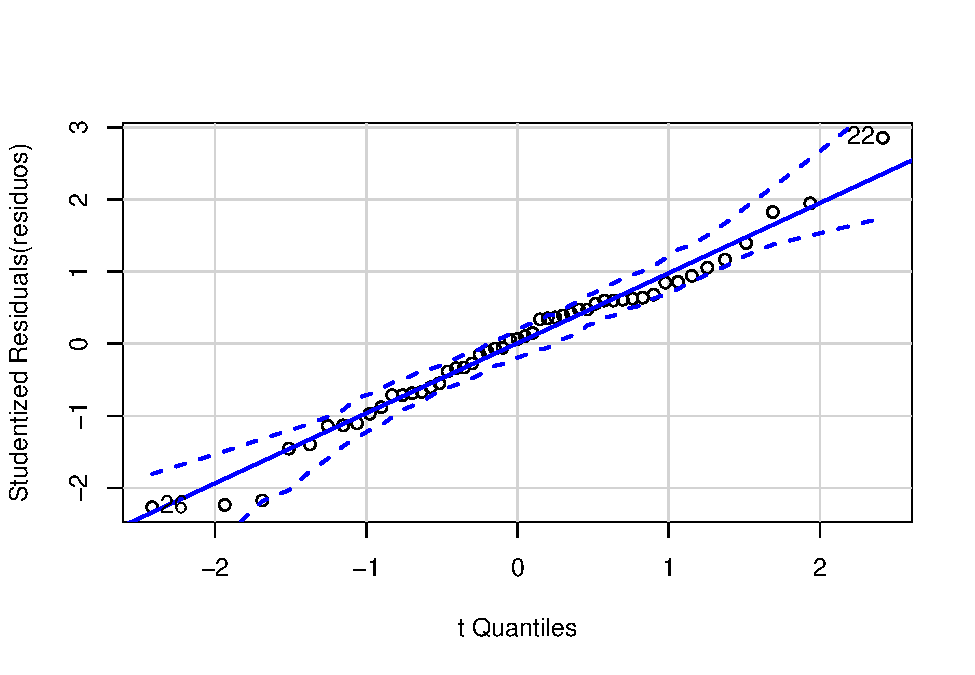
\includegraphics{livro_r_ecologia_files/figure-latex/unnamed-chunk-1-1.pdf}

\hypertarget{interpretauxe7uxe3o-dos-resultados}{%
\subsection{Interpretação dos resultados}\label{interpretauxe7uxe3o-dos-resultados}}

Neste exemplo, foram registrados 166 indivíduos na MC\_Tenentes, 413 na MC\_Talhadinho e 223 na FF\_Experimental. Lembrando, você não pode comparar a riqueza de espécies observada diretamente: 15 espécies na MC\_Tenentes, 17 espécies na MC\_Talhadinho, e 13 espécies no FF\_Experimental. A comparação da riqueza de espécies entre as comunidades deve ser feita com base na riqueza de espécies estimada que é calculada com base no número de indivíduos da comunidade com menor abundância (166 indivíduos). Olhando o gráfico é possível perceber que a riqueza de espécies de morcegos estimada não é diferente entre os três fragmentos florestais quando corrigimos o problema da abundância pela rarefação. A interpretação é feita com base no intervalo de confiança de 95\%. As curvas serão diferentes quando os intervalos de confiança não se sobreporem (Chao et al.~2014). Percebam que está abordagem, além da interpolação (rarefação), também realiza extrapolações que podem ser usadas para estimar o número de espécies caso o esforço de coleta fosse maior. Este é o assunto do nosso próximo capítulo.

~

\hypertarget{exemplo-pruxe1tico-2---rarefauxe7uxe3o}{%
\section{Exemplo prático 2 - Rarefação}\label{exemplo-pruxe1tico-2---rarefauxe7uxe3o}}

\hypertarget{explicauxe7uxe3o-1}{%
\subsection{Explicação}\label{explicauxe7uxe3o-1}}

\textbf{Explicação dos dados}

Neste exemplo iremos comparar o número de espécies de anuros e répteis (serptentes e lagartos) usando informações dos indivíduos depositados em coleções científicas e coletas de campo (da Silva et al.~2017).

\textbf{Pergunta:}

\begin{quote}
A riqueza de espécies de anuros e répteis é maior em coleções científicas do que nas coletas de campo?
\end{quote}

\textbf{Predições}

\begin{quote}
O número de espécies será maior em coleções científicas devido ao maior esforço amostral (i.e.~maior variação temporal para depositar os indíviduos e maior número de pessoas contribuindo com as informações de diferentes estudos e/ou coletas esporádicas).
\end{quote}

\textbf{Variáveis}

\begin{itemize}
\tightlist
\item
  Variáveis preditoras

  \begin{itemize}
  \tightlist
  \item
    matriz ou dataframe com as abundâncias das espécies de anuros e répteis (planilhas separadas) registradas em coleções científicas e coletas de campo.
  \end{itemize}
\end{itemize}

\textbf{Checklist}

\begin{itemize}
\tightlist
\item
  Verificar se a sua matriz ou dataframe estão com as espécies nas linhas e a fonte dos dados nas colunas.
\end{itemize}

\hypertarget{anuxe1lise-1}{%
\subsection{Análise}\label{anuxe1lise-1}}

Calculo da rarefação para os dados de répteis

\begin{Shaded}
\begin{Highlighting}[]
\KeywordTok{library}\NormalTok{(iNEXT)}

\NormalTok{rarefacao_repteis <-}\StringTok{ }\NormalTok{rarefacao_repteis}
\NormalTok{resultados_repteis <-}\StringTok{ }\KeywordTok{iNEXT}\NormalTok{(rarefacao_repteis, }\DataTypeTok{q =} \DecValTok{0}\NormalTok{, }\DataTypeTok{datatype =} \StringTok{"abundance"}\NormalTok{, }\DataTypeTok{endpoint =} \DecValTok{200}\NormalTok{)}

\CommentTok{# Visualizar os resultados }
\KeywordTok{ggiNEXT}\NormalTok{(resultados_repteis, }\DataTypeTok{type =} \DecValTok{1}\NormalTok{)}
\end{Highlighting}
\end{Shaded}

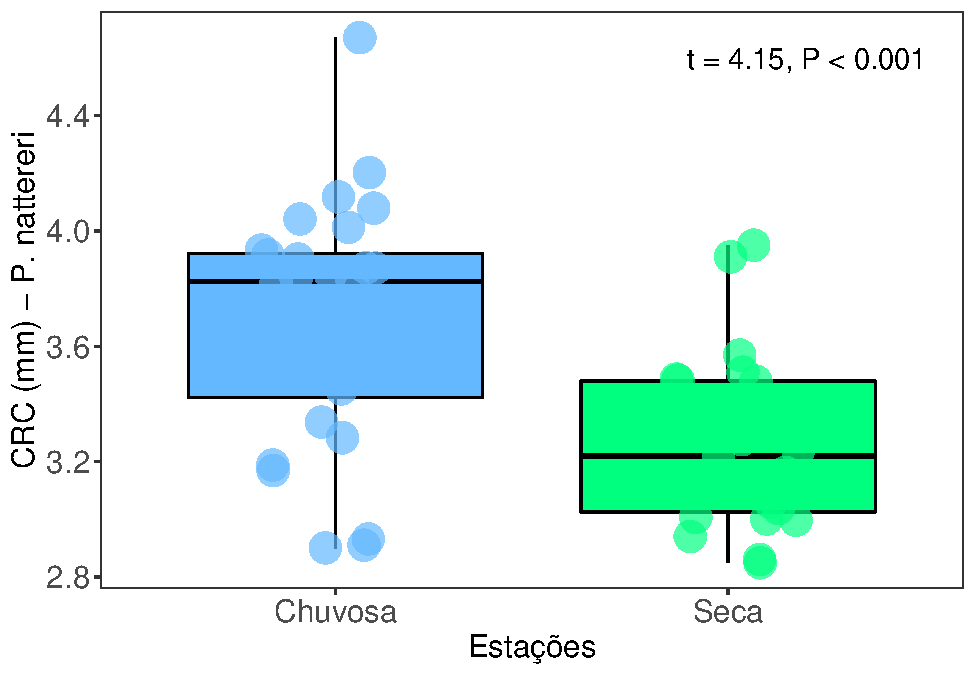
\includegraphics{livro_r_ecologia_files/figure-latex/unnamed-chunk-2-1.pdf}

\hypertarget{interpretauxe7uxe3o-dos-resultados-1}{%
\subsection{Interpretação dos resultados}\label{interpretauxe7uxe3o-dos-resultados-1}}

Neste exemplo,foram registradas oito espécies de répteis nas coletas de campo (40 indivíduos) e 28 espécies nas coleções científicas (77 indivíduos). Com base na rarefação, concluímos que a riqueza de espécies de répteis obtida nas coleções científicas é 2,5 vezes maior do que a obtida em coletas de campo.

~

Calculo da rarefação para os dados dos anuros

\begin{Shaded}
\begin{Highlighting}[]
\KeywordTok{library}\NormalTok{(iNEXT)}

\NormalTok{rarefacao_anuros <-}\StringTok{ }\NormalTok{rarefacao_anuros}
\NormalTok{resultados_anuros <-}\StringTok{ }\KeywordTok{iNEXT}\NormalTok{(rarefacao_anuros, }\DataTypeTok{q =} \DecValTok{0}\NormalTok{, }\DataTypeTok{datatype =} \StringTok{"abundance"}\NormalTok{, }\DataTypeTok{endpoint =} \DecValTok{800}\NormalTok{)}

\CommentTok{# Visualizar os resultados }
\KeywordTok{ggiNEXT}\NormalTok{(resultados_anuros, }\DataTypeTok{type =} \DecValTok{1}\NormalTok{, }\DataTypeTok{grey =} \OtherTok{TRUE}\NormalTok{)}
\end{Highlighting}
\end{Shaded}

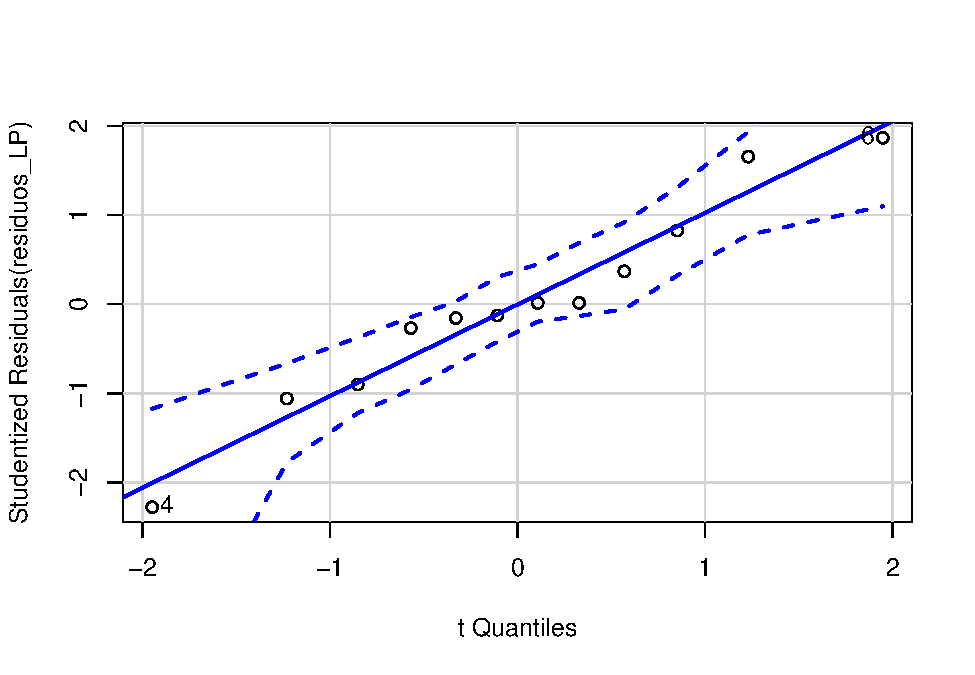
\includegraphics{livro_r_ecologia_files/figure-latex/unnamed-chunk-3-1.pdf}

\textbf{Interpretação dos resultados}

Neste exemplo,foram registradas 21 espécies de anuros nas coletas de campo (709 indivíduos) e 12 espécies nas coleções científicas (37 indivíduos). Com base na rarefação, concluímos que não há diferença entre a riqueza de espécies de anuros obtida em coletas de campo e coleções científicas.

~

\hypertarget{para-se-aprofundar}{%
\section{Para se aprofundar}\label{para-se-aprofundar}}

\begin{itemize}
\item
  Recomendamos aos interessados que olhem a página do \href{http://viceroy.eeb.uconn.edu/estimates}{EstimateS software} e baixem o manual do usuário que contém informações detalhadas sobre os índices de rarefação.Este site foi criado e é mantido pelo Dr.~Robert K. Colwell, um dos maiores especialistas do mundo em estimativas da biodiversidade
\item
  Recomendamos também o livro Magurran \& McGill (2010) - Biological Diversity Frontiers in Measurement and Assessment.
\end{itemize}

\hypertarget{estimadores-de-riqueza}{%
\chapter{Estimadores de Riqueza}\label{estimadores-de-riqueza}}

\hypertarget{backgorund-da-anuxe1lise}{%
\section{Backgorund da análise}\label{backgorund-da-anuxe1lise}}

Uma vez que determinar o número total de espécies numa área é praticamente impossível, principalmente em regiões com alta riqueza de espécies, os estimadores são úteis para extrapolar a riqueza observada e tentar estimar a riqueza total através de uma amostra incompleta de uma comunidade biológica (Walther \& Moore 2005). Neste capítulo serão considerados os estimadores não paramétricos que usam informações da frequencia de espécies raras na comunidade (Gotelli \& Chao 2013). Isto porque tanto os testes paramétricos que tentam determinar os parâmetros de uma curva usando o formato da curva de acumulação de espécies (e.g.~equação logística, Michaelis-Menten) quanto os testes que usam a frequencia do número de indivíduos para enquadrá-las em uma das distribuições de abundância das espécies (e.g.~distribuições log-séries, log-normal) não funcionam muito bem com dados empíricos (Gotelli \& Chao 2013). Para mais detalhes sobre os testes paramétricos veja Magurran (2004) e Colwell (2019).

\begin{quote}
\hypertarget{quatro-caracteruxedsticas-para-um-bom-estimador-de-riqueza-chazdon-et-al.-1998-horter-et-al.-2006}{%
\subsubsection{Quatro características para um bom estimador de riqueza (Chazdon et al.~1998; Horter et al.~2006):}\label{quatro-caracteruxedsticas-para-um-bom-estimador-de-riqueza-chazdon-et-al.-1998-horter-et-al.-2006}}

\begin{itemize}
\tightlist
\item
  Independência do tamanho da amostra (quantidade de esforço amostral realizado);
\item
  Insensibilidade a diferentes padrões de distribuições (diferentes equitabilidades);
\item
  Insensibilidade em relação à ordem das amostragens;
\item
  Insensibilidade à heterogeneidade entre as amostras usadas entre estudos.
\end{itemize}
\end{quote}

\hypertarget{estimadores-baseados-na-abunduxe2ncia-das-espuxe9cies}{%
\section{Estimadores baseados na abundância das espécies}\label{estimadores-baseados-na-abunduxe2ncia-das-espuxe9cies}}

\hypertarget{chao-1---chao-1984-1987}{%
\subsection{CHAO 1 - (Chao 1984, 1987):}\label{chao-1---chao-1984-1987}}

Estimador simples do número absoluto de espécies em uma comunidade. É baseado no número de espécies raras dentro de uma amostra.

\begin{quote}
\[Chao_{1} = S_{obs} + \left(\frac{n-1}{n}\right)\frac{F_1(F_1-1)}{2(F_2+1)}\]
\end{quote}

onde:

\begin{itemize}
\item
  Sobs = o número de espécies na comunidade,
\item
  \emph{n} = número de amostras,
\item
  F1 = número de espécies observadas com abundância de um indivíduo (espécies \emph{singleton}),
\item
  F2 = número de espécies observadas com abundância de dois indivíduos (espécies \emph{doubletons}).
\end{itemize}

O valor de Chao 1 é máximo quando todas as espécies menos uma são únicas (\emph{singleton}). Neste caso, a riqueza estimada é aproximadamente o dobro da riqueza observada.

~

\hypertarget{exemplo-pruxe1tico---chao-1}{%
\subsubsection{Exemplo prático - Chao 1}\label{exemplo-pruxe1tico---chao-1}}

\hypertarget{explicauxe7uxe3o-dos-dados}{%
\paragraph{Explicação dos dados}\label{explicauxe7uxe3o-dos-dados}}

Neste exemplo usaremos os dados de 17 espécies de anuros amostradas em 14 dias de coletas de campo em um habitat reprodutivo localizado na região noroeste do estado de São Paulo, Brasil.

\textbf{Pergunta:}

\begin{quote}
Quantas espécies a mais poderiam ser amostradas caso aumentasse o esforço amostral?
\end{quote}

\textbf{Predições}

\begin{quote}
\begin{itemize}
\tightlist
\item
  O número de espécies estimadas é similar ao número de espécies observada;
\item
  O número de espécies estimadas é maior do que o número de espécies observada.
\end{itemize}
\end{quote}

\textbf{Variáveis}

\begin{itemize}
\tightlist
\item
  Variáveis preditoras

  \begin{itemize}
  \tightlist
  \item
    matriz ou vetor com as abundâncias das espécies de anuros registradas em uma habitat reprodutivo
  \end{itemize}
\end{itemize}

\textbf{Checklist}

\begin{itemize}
\tightlist
\item
  Verificar se a sua matriz está com as espécies nas colunas e as amostragens nas linhas
\item
  Verificar se os dados são de abundância e não presença e ausência
\end{itemize}

\hypertarget{anuxe1lise-2}{%
\subsection{Análise}\label{anuxe1lise-2}}

Calculo do estimador de riqueza - Chao 1

\begin{Shaded}
\begin{Highlighting}[]
\KeywordTok{library}\NormalTok{(ecodados)}
\KeywordTok{library}\NormalTok{(vegan)}
\NormalTok{dados_coleta <-}\StringTok{ }\NormalTok{poca_anuros}
\NormalTok{est_chao1 <-}\StringTok{ }\KeywordTok{estaccumR}\NormalTok{(dados_coleta, }\DataTypeTok{permutations =} \DecValTok{100}\NormalTok{)}
\KeywordTok{summary}\NormalTok{(est_chao1, }\DataTypeTok{display =} \StringTok{"chao"}\NormalTok{)}
\end{Highlighting}
\end{Shaded}

\begin{verbatim}
## $chao
##         N      Chao    2.5%    97.5%  Std.Dev
## Dia_12  1  6.651667  3.0000 12.33333 2.679640
## Dia_10  2  9.904167  6.0000 15.00000 2.655262
## Dia_3   3 11.607667  8.0000 17.76250 2.674637
## Dia_1   4 12.605833  9.0000 18.05000 2.526233
## Dia_4   5 13.430000  9.0000 18.52500 2.579399
## Dia_6   6 14.198333 10.0000 20.00000 2.652286
## Dia_9   7 15.155000 11.0000 22.00000 2.813533
## Dia_8   8 16.200000 11.0000 22.00000 2.840010
## Dia_2   9 16.840000 12.0000 22.00000 2.898868
## Dia_5  10 17.570000 13.0000 22.00000 2.651491
## Dia_14 11 18.290000 13.4750 22.00000 2.408088
## Dia_11 12 18.885000 14.7375 22.00000 2.106813
## Dia_7  13 19.405000 15.5000 20.00000 1.419018
## Dia_13 14 20.000000 20.0000 20.00000 0.000000
## 
## attr(,"class")
## [1] "summary.poolaccum"
\end{verbatim}

Visualizar os resultados com intervalo de confiança de 95\%.

\begin{Shaded}
\begin{Highlighting}[]
\KeywordTok{library}\NormalTok{(ggplot2)}
\CommentTok{# preparando os dados para fazer o gráfico}
\NormalTok{resultados <-}\StringTok{ }\KeywordTok{summary}\NormalTok{(est_chao1, }\DataTypeTok{display =} \KeywordTok{c}\NormalTok{(}\StringTok{"S"}\NormalTok{, }\StringTok{"chao"}\NormalTok{))}
\NormalTok{res_chao <-}\StringTok{ }\KeywordTok{cbind}\NormalTok{(resultados}\OperatorTok{$}\NormalTok{chao[,}\DecValTok{1}\OperatorTok{:}\DecValTok{4}\NormalTok{], resultados}\OperatorTok{$}\NormalTok{S[,}\DecValTok{2}\OperatorTok{:}\DecValTok{4}\NormalTok{])}
\NormalTok{res_chao <-}\StringTok{ }\KeywordTok{as.data.frame}\NormalTok{(res_chao)}
\KeywordTok{colnames}\NormalTok{(res_chao) <-}\StringTok{ }\KeywordTok{c}\NormalTok{(}\StringTok{"Amostras"}\NormalTok{, }\StringTok{"Chao"}\NormalTok{, }\StringTok{"C_inferior"}\NormalTok{, }\StringTok{"C_superior"}\NormalTok{, }\StringTok{"Riqueza"}\NormalTok{,}
                        \StringTok{"R_inferior"}\NormalTok{, }\StringTok{"R_superior"}\NormalTok{)}

\CommentTok{# comando para o gráfico}
\KeywordTok{ggplot}\NormalTok{(res_chao, }\KeywordTok{aes}\NormalTok{(}\DataTypeTok{y =}\NormalTok{ Riqueza, }\DataTypeTok{x =}\NormalTok{ Amostras)) }\OperatorTok{+}
\StringTok{  }\KeywordTok{geom_point}\NormalTok{(}\KeywordTok{aes}\NormalTok{(}\DataTypeTok{y =}\NormalTok{ Chao, }\DataTypeTok{x =}\NormalTok{ Amostras }\OperatorTok{+}\StringTok{ }\FloatTok{0.1}\NormalTok{), }\DataTypeTok{size =} \DecValTok{5}\NormalTok{, }\DataTypeTok{color =} \StringTok{"blue"}\NormalTok{, }\DataTypeTok{alpha =} \DecValTok{1}\NormalTok{) }\OperatorTok{+}
\StringTok{  }\KeywordTok{geom_point}\NormalTok{(}\KeywordTok{aes}\NormalTok{(}\DataTypeTok{y =}\NormalTok{ Riqueza, }\DataTypeTok{x =}\NormalTok{ Amostras), }\DataTypeTok{size =} \DecValTok{5}\NormalTok{, }\DataTypeTok{color =} \StringTok{"red"}\NormalTok{, }\DataTypeTok{alpha =} \DecValTok{1}\NormalTok{) }\OperatorTok{+}
\StringTok{  }\KeywordTok{geom_line}\NormalTok{ (}\KeywordTok{aes}\NormalTok{(}\DataTypeTok{y =}\NormalTok{ Chao, }\DataTypeTok{x =}\NormalTok{ Amostras), }\DataTypeTok{color =} \StringTok{"blue"}\NormalTok{) }\OperatorTok{+}
\StringTok{  }\KeywordTok{geom_line}\NormalTok{ (}\KeywordTok{aes}\NormalTok{(}\DataTypeTok{y =}\NormalTok{ Riqueza, }\DataTypeTok{x =}\NormalTok{ Amostras), }\DataTypeTok{color =} \StringTok{"red"}\NormalTok{) }\OperatorTok{+}
\StringTok{  }\KeywordTok{geom_linerange}\NormalTok{(}\KeywordTok{aes}\NormalTok{(}\DataTypeTok{ymin =}\NormalTok{ C_inferior, }\DataTypeTok{ymax =}\NormalTok{ C_superior, }\DataTypeTok{x =}\NormalTok{ Amostras }\OperatorTok{+}\StringTok{ }\FloatTok{0.1}\NormalTok{),}
 \DataTypeTok{color =} \StringTok{"blue"}\NormalTok{) }\OperatorTok{+}
\StringTok{  }\KeywordTok{geom_linerange}\NormalTok{(}\KeywordTok{aes}\NormalTok{(}\DataTypeTok{ymin =}\NormalTok{ R_inferior, }\DataTypeTok{ymax =}\NormalTok{ R_superior, }\DataTypeTok{x =}\NormalTok{ Amostras), }\DataTypeTok{color =} \StringTok{"red"}\NormalTok{) }\OperatorTok{+}
\StringTok{  }\KeywordTok{ylab}\NormalTok{ (}\StringTok{"Estimador de riqueza - Chao 1"}\NormalTok{) }\OperatorTok{+}
\StringTok{  }\KeywordTok{xlab}\NormalTok{ (}\StringTok{"Número de amostras"}\NormalTok{) }\OperatorTok{+}
\StringTok{  }\KeywordTok{scale_x_continuous}\NormalTok{(}\DataTypeTok{limits =} \KeywordTok{c}\NormalTok{(}\DecValTok{1}\NormalTok{,}\DecValTok{15}\NormalTok{), }\DataTypeTok{breaks=}\KeywordTok{seq}\NormalTok{(}\DecValTok{1}\NormalTok{,}\DecValTok{15}\NormalTok{,}\DecValTok{1}\NormalTok{)) }\OperatorTok{+}
\StringTok{  }\KeywordTok{geom_point}\NormalTok{(}\DataTypeTok{y=} \FloatTok{7.5}\NormalTok{, }\DataTypeTok{x =} \DecValTok{9}\NormalTok{, }\DataTypeTok{size =} \DecValTok{5}\NormalTok{, }\DataTypeTok{color =} \StringTok{"blue"}\NormalTok{, }\DataTypeTok{alpha =} \DecValTok{1}\NormalTok{) }\OperatorTok{+}\StringTok{ }
\StringTok{  }\KeywordTok{geom_point}\NormalTok{(}\DataTypeTok{y=} \FloatTok{5.9}\NormalTok{, }\DataTypeTok{x =} \DecValTok{9}\NormalTok{, }\DataTypeTok{size =} \DecValTok{5}\NormalTok{, }\DataTypeTok{color =} \StringTok{"red"}\NormalTok{, }\DataTypeTok{alpha =} \DecValTok{1}\NormalTok{) }\OperatorTok{+}\StringTok{ }
\StringTok{  }\KeywordTok{geom_label}\NormalTok{( }\DataTypeTok{y =} \FloatTok{7.5}\NormalTok{, }\DataTypeTok{x =} \DecValTok{12}\NormalTok{, }\DataTypeTok{label =} \StringTok{"Riqueza estimada - Chao 1"}\NormalTok{) }\OperatorTok{+}
\StringTok{  }\KeywordTok{geom_label}\NormalTok{( }\DataTypeTok{y =} \FloatTok{5.9}\NormalTok{, }\DataTypeTok{x =} \FloatTok{11.3}\NormalTok{, }\DataTypeTok{label =} \StringTok{"Riqueza observada"}\NormalTok{)}
\end{Highlighting}
\end{Shaded}

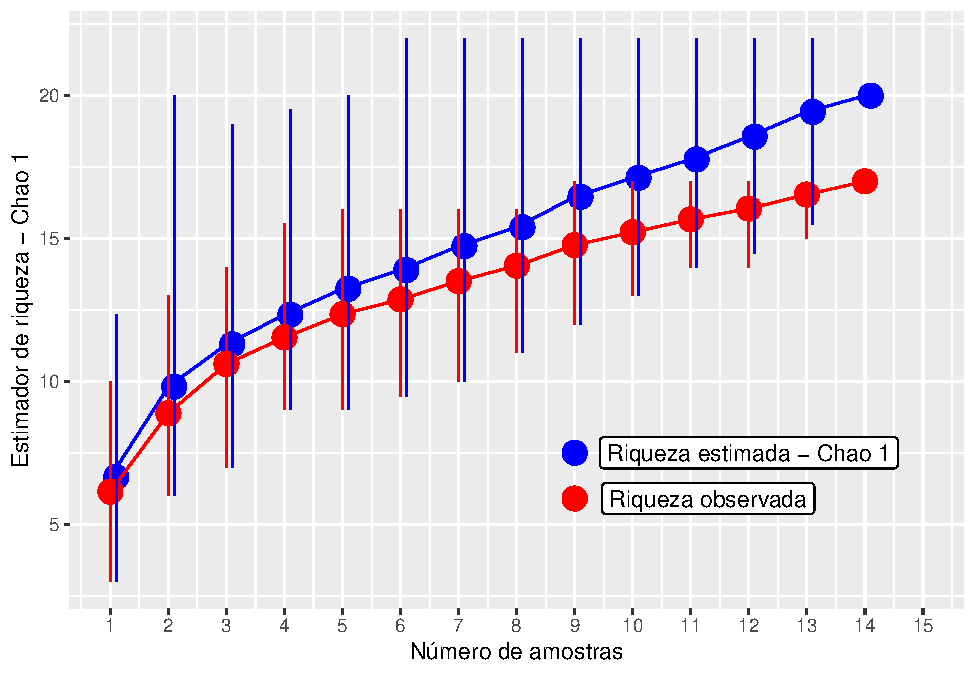
\includegraphics{livro_r_ecologia_files/figure-latex/unnamed-chunk-5-1.pdf}

\hypertarget{interpretauxe7uxe3o-dos-resultados-2}{%
\subsubsection{Interpretação dos resultados}\label{interpretauxe7uxe3o-dos-resultados-2}}

Com base no número de espécies raras (\emph{singletons} e \emph{doubletons}), o estimador Chao 1 indica a possibilidade de encontrarmos mais três espécies caso o esforço amostral fosse maior e não mostra tendência de estabilização da curva em uma assíntota.

\hypertarget{ace---abundance-based-coverage-estimador-chao-lee-1992-chao-et-al.-2000}{%
\subsection{\texorpdfstring{ACE - \emph{Abundance-based Coverage Estimador} (Chao \& Lee 1992, Chao et al.~2000):}{ACE - Abundance-based Coverage Estimador (Chao \& Lee 1992, Chao et al.~2000):}}\label{ace---abundance-based-coverage-estimador-chao-lee-1992-chao-et-al.-2000}}

Este método trabalha com a abundância das espécies raras (i.e.~abundância baixa). Entretanto, diferente do estimador anterior, esse método permite ao pesquisador determinar os limites para os quais uma espécie seja considerada rara. Em geral, são consideradas raras espécies com abundância entre 1 e 10 indivíduos. A riqueza estimada pode variar conforme se aumente ou diminua o limiar de abundância, e infelizmente não existem critérios biológicos definidos para a escolha do melhor intervalo.

\begin{quote}
\[ACE = S_{abund} + \frac{S_{rare}}{C_{ace}} + \frac{F_1}{C_{ace}}Y_{ace}^2\]
\end{quote}

onde:

\begin{quote}
\[Y_{ace}^2 = max \left[\frac{S_{rare}}{C_{ace}}\frac{\sum_{i=i}^{10}i(i-1)F1}{(N_{rare})({N_{rare} - 1)}}-1,0\right]\]
\end{quote}

\begin{quote}
\[C_{ace} = 1 - \frac{F1}{N_{rare}}\]
\end{quote}

\begin{quote}
\[N_{rare} = \sum_{i=1}^{10}iF_i\]
\end{quote}

Não precisa fazer cara feia, é óbvio que iremos usar o programa para fazer esses cálculos.

~

\hypertarget{exemplo-pruxe1tico---ace}{%
\subsubsection{Exemplo prático - ACE}\label{exemplo-pruxe1tico---ace}}

\hypertarget{explicauxe7uxe3o-dos-dados-1}{%
\paragraph{Explicação dos dados}\label{explicauxe7uxe3o-dos-dados-1}}

Usaremos os mesmos dados de 17 espécies de anuros amostradas em 14 dias de coletas de campo em um habitat reprodutivo localizado na região noroeste do estado de São Paulo, Brasil.

\textbf{Pergunta:}

\begin{quote}
Quantas espécies a mais poderiam ser amostradas caso aumentasse o esforço amostral?
\end{quote}

\textbf{Predições}

\begin{quote}
\begin{itemize}
\tightlist
\item
  O número de espécies estimadas é similar ao número de espécies observada;
\item
  O número de espécies estimadas é maior do que o número de espécies observada.
\end{itemize}
\end{quote}

\textbf{Variáveis}

\begin{itemize}
\tightlist
\item
  Variáveis preditoras

  \begin{itemize}
  \tightlist
  \item
    matriz ou vetor com as abundâncias das espécies de anuros registradas em uma habitat reprodutivo
  \end{itemize}
\end{itemize}

\textbf{Checklist}

\begin{itemize}
\tightlist
\item
  Verificar se a sua matriz está com as espécies nas colunas e as amostragens nas linhas
\item
  Verificar se os dados são de abundância e não presença e ausência
\end{itemize}

\hypertarget{anuxe1lise-3}{%
\subsection{Análise}\label{anuxe1lise-3}}

Calculo do estimador de riqueza - ACE

\begin{Shaded}
\begin{Highlighting}[]
\KeywordTok{library}\NormalTok{(vegan)}
\NormalTok{dados_coleta <-}\StringTok{ }\NormalTok{poca_anuros}
\NormalTok{est_ace <-}\StringTok{ }\KeywordTok{estaccumR}\NormalTok{(dados_coleta, }\DataTypeTok{permutations =} \DecValTok{100}\NormalTok{)}
\KeywordTok{summary}\NormalTok{(est_ace, }\DataTypeTok{display =} \StringTok{"ace"}\NormalTok{)}
\end{Highlighting}
\end{Shaded}

\begin{verbatim}
## $ace
##         N       ACE      2.5%    97.5%  Std.Dev
## Dia_13  1  7.612776  3.761224 13.71429 2.853244
## Dia_2   2  9.733455  6.000000 15.74635 2.561675
## Dia_14  3 11.259911  8.000000 15.87885 2.078870
## Dia_7   4 12.425328  8.121225 18.54988 2.663095
## Dia_12  5 13.553731  8.475000 19.87776 2.973525
## Dia_10  6 14.446920  9.167937 20.02742 2.894626
## Dia_9   7 15.050844 10.000000 20.44469 2.805688
## Dia_6   8 15.997108 10.000000 22.76955 3.258119
## Dia_1   9 17.809288 12.000000 24.93470 3.776383
## Dia_8  10 19.377831 13.005455 25.09679 3.997948
## Dia_3  11 21.046964 13.686710 25.72368 3.862266
## Dia_4  12 22.454068 16.144275 25.72368 3.404189
## Dia_5  13 23.841765 17.676471 25.72368 2.416507
## Dia_11 14 24.703704 24.703704 24.70370 0.000000
## 
## attr(,"class")
## [1] "summary.poolaccum"
\end{verbatim}

Visualizar os resultados com intervalo de confiança de 95\%

\begin{Shaded}
\begin{Highlighting}[]
\KeywordTok{library}\NormalTok{(ggplot2)}
\CommentTok{# preparando os dados para fazer o gráfico}
\NormalTok{resultados_ace <-}\StringTok{ }\KeywordTok{summary}\NormalTok{(est_ace, }\DataTypeTok{display =} \KeywordTok{c}\NormalTok{(}\StringTok{"S"}\NormalTok{, }\StringTok{"ace"}\NormalTok{))}
\NormalTok{res_ace <-}\StringTok{ }\KeywordTok{cbind}\NormalTok{(resultados_ace}\OperatorTok{$}\NormalTok{ace[,}\DecValTok{1}\OperatorTok{:}\DecValTok{4}\NormalTok{], resultados_ace}\OperatorTok{$}\NormalTok{S[,}\DecValTok{2}\OperatorTok{:}\DecValTok{4}\NormalTok{])}
\NormalTok{res_ace <-}\StringTok{ }\KeywordTok{as.data.frame}\NormalTok{(res_ace)}
\KeywordTok{colnames}\NormalTok{(res_ace) <-}\StringTok{ }\KeywordTok{c}\NormalTok{(}\StringTok{"Amostras"}\NormalTok{, }\StringTok{"ACE"}\NormalTok{, }\StringTok{"ACE_inferior"}\NormalTok{, }\StringTok{"ACE_superior"}\NormalTok{, }\StringTok{"Riqueza"}\NormalTok{,}
                        \StringTok{"R_inferior"}\NormalTok{, }\StringTok{"R_superior"}\NormalTok{)}

\CommentTok{# comando para o gráfico}
\KeywordTok{ggplot}\NormalTok{(res_ace, }\KeywordTok{aes}\NormalTok{(}\DataTypeTok{y =}\NormalTok{ Riqueza, }\DataTypeTok{x =}\NormalTok{ Amostras)) }\OperatorTok{+}
\StringTok{  }\KeywordTok{geom_point}\NormalTok{(}\KeywordTok{aes}\NormalTok{(}\DataTypeTok{y =}\NormalTok{ ACE, }\DataTypeTok{x =}\NormalTok{ Amostras }\OperatorTok{+}\StringTok{ }\FloatTok{0.1}\NormalTok{), }\DataTypeTok{size =} \DecValTok{5}\NormalTok{, }\DataTypeTok{color =} \StringTok{"blue"}\NormalTok{, }\DataTypeTok{alpha =} \DecValTok{1}\NormalTok{) }\OperatorTok{+}
\StringTok{  }\KeywordTok{geom_point}\NormalTok{(}\KeywordTok{aes}\NormalTok{(}\DataTypeTok{y =}\NormalTok{ Riqueza, }\DataTypeTok{x =}\NormalTok{ Amostras), }\DataTypeTok{size =} \DecValTok{5}\NormalTok{, }\DataTypeTok{color =} \StringTok{"red"}\NormalTok{, }\DataTypeTok{alpha =} \DecValTok{1}\NormalTok{) }\OperatorTok{+}
\StringTok{  }\KeywordTok{geom_line}\NormalTok{ (}\KeywordTok{aes}\NormalTok{(}\DataTypeTok{y =}\NormalTok{ ACE, }\DataTypeTok{x =}\NormalTok{ Amostras), }\DataTypeTok{color =} \StringTok{"blue"}\NormalTok{) }\OperatorTok{+}
\StringTok{  }\KeywordTok{geom_line}\NormalTok{ (}\KeywordTok{aes}\NormalTok{(}\DataTypeTok{y =}\NormalTok{ Riqueza, }\DataTypeTok{x =}\NormalTok{ Amostras), }\DataTypeTok{color =} \StringTok{"red"}\NormalTok{) }\OperatorTok{+}
\StringTok{  }\KeywordTok{geom_linerange}\NormalTok{(}\KeywordTok{aes}\NormalTok{(}\DataTypeTok{ymin =}\NormalTok{ ACE_inferior, }\DataTypeTok{ymax =}\NormalTok{ ACE_superior, }\DataTypeTok{x =}\NormalTok{ Amostras }\OperatorTok{+}\StringTok{ }\FloatTok{0.1}\NormalTok{),}
 \DataTypeTok{color =} \StringTok{"blue"}\NormalTok{) }\OperatorTok{+}
\StringTok{  }\KeywordTok{geom_linerange}\NormalTok{(}\KeywordTok{aes}\NormalTok{(}\DataTypeTok{ymin =}\NormalTok{ R_inferior, }\DataTypeTok{ymax =}\NormalTok{ R_superior, }\DataTypeTok{x =}\NormalTok{ Amostras), }\DataTypeTok{color =} \StringTok{"red"}\NormalTok{) }\OperatorTok{+}
\StringTok{  }\KeywordTok{ylab}\NormalTok{ (}\StringTok{"Estimador de riqueza - ACE"}\NormalTok{) }\OperatorTok{+}
\StringTok{  }\KeywordTok{xlab}\NormalTok{ (}\StringTok{"Número de amostras"}\NormalTok{) }\OperatorTok{+}
\StringTok{  }\KeywordTok{scale_x_continuous}\NormalTok{(}\DataTypeTok{limits =} \KeywordTok{c}\NormalTok{(}\DecValTok{1}\NormalTok{,}\DecValTok{15}\NormalTok{), }\DataTypeTok{breaks=}\KeywordTok{seq}\NormalTok{(}\DecValTok{1}\NormalTok{,}\DecValTok{15}\NormalTok{,}\DecValTok{1}\NormalTok{)) }\OperatorTok{+}
\StringTok{  }\KeywordTok{geom_point}\NormalTok{(}\DataTypeTok{y=} \FloatTok{7.5}\NormalTok{, }\DataTypeTok{x =} \DecValTok{9}\NormalTok{, }\DataTypeTok{size =} \DecValTok{5}\NormalTok{, }\DataTypeTok{color =} \StringTok{"blue"}\NormalTok{, }\DataTypeTok{alpha =} \DecValTok{1}\NormalTok{) }\OperatorTok{+}\StringTok{ }
\StringTok{  }\KeywordTok{geom_point}\NormalTok{(}\DataTypeTok{y=} \FloatTok{5.9}\NormalTok{, }\DataTypeTok{x =} \DecValTok{9}\NormalTok{, }\DataTypeTok{size =} \DecValTok{5}\NormalTok{, }\DataTypeTok{color =} \StringTok{"red"}\NormalTok{, }\DataTypeTok{alpha =} \DecValTok{1}\NormalTok{) }\OperatorTok{+}\StringTok{ }
\StringTok{  }\KeywordTok{geom_label}\NormalTok{( }\DataTypeTok{y =} \FloatTok{7.5}\NormalTok{, }\DataTypeTok{x =} \FloatTok{11.7}\NormalTok{, }\DataTypeTok{label =} \StringTok{"Riqueza estimada - ACE"}\NormalTok{) }\OperatorTok{+}
\StringTok{  }\KeywordTok{geom_label}\NormalTok{( }\DataTypeTok{y =} \FloatTok{5.9}\NormalTok{, }\DataTypeTok{x =} \FloatTok{11.3}\NormalTok{, }\DataTypeTok{label =} \StringTok{"Riqueza observada"}\NormalTok{)}
\end{Highlighting}
\end{Shaded}

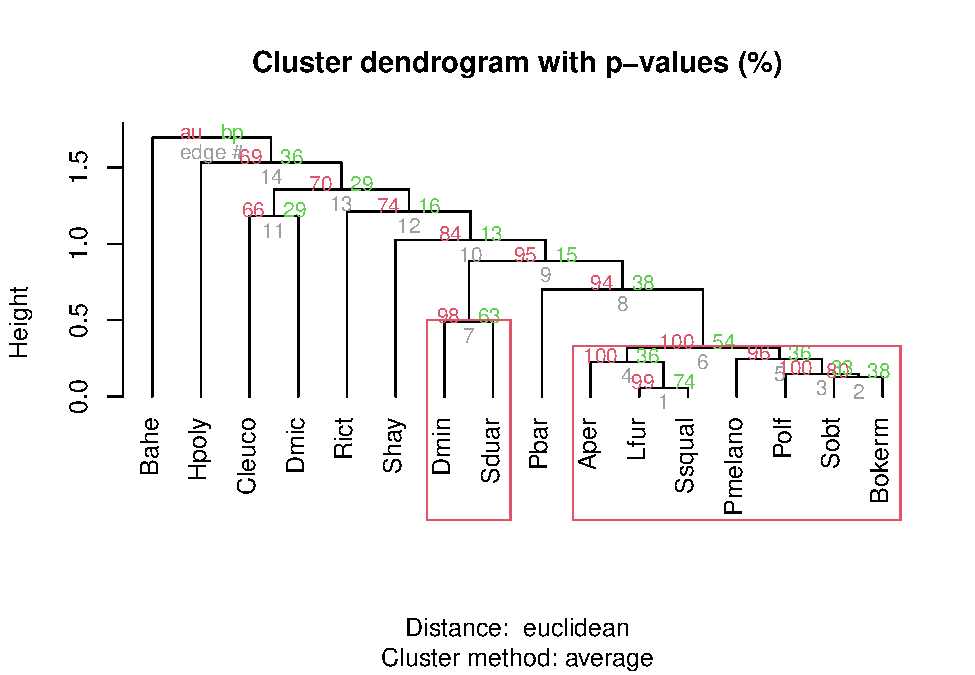
\includegraphics{livro_r_ecologia_files/figure-latex/unnamed-chunk-7-1.pdf}

\hypertarget{interpretauxe7uxe3o-dos-resultados-3}{%
\subsubsection{Interpretação dos resultados}\label{interpretauxe7uxe3o-dos-resultados-3}}

Com base no número de espécies raras (abundância menor que 10 indivíduos - \emph{default}), o estimador ACE indica a possibilidade de encontrarmos mais sete espécies caso o esforço amostral fosse maior e não mostrou tendência de estabilição da curva em uma assíntota.

\hypertarget{estimadores-baseados-na-inciduxeancia-das-espuxe9cies}{%
\section{Estimadores baseados na incidência das espécies}\label{estimadores-baseados-na-inciduxeancia-das-espuxe9cies}}

\hypertarget{chao-2---chao-1987}{%
\subsection{CHAO 2 - (Chao 1987):}\label{chao-2---chao-1987}}

De acordo com Anne Chao, o estimador Chao 1 pode ser modificado para uso com dados de presença/ausência levando em conta a distribuição das espécies entre amostras. Neste caso é
necessário somente conhecer o número de espécies encontradas em somente uma amostra e o
número de espécies encontradas exatamente em duas amostras. Essa variação ficou denominada como
Chao 2:

\begin{quote}
\[Chao_{2} = S_{obs} + \left(\frac{m-1}{m}\right)\left(\frac{Q_1(Q_1-1)}{2(Q_2 + 1}\right)\]
\end{quote}

onde:

\begin{itemize}
\item
  Sobs = o número de espécies na comunidade,
\item
  \emph{m} = número de amostragens,
\item
  Q1 = número de espécies observadas em uma amostragem (espécies \emph{uniques}),
\item
  Q2 = número de espécies observadas em duas amostragens (espécies \emph{duplicates}).
\end{itemize}

O valor de Chao2 é máximo quando as espécies menos uma são únicas (\emph{uniques}). Neste caso, a riqueza estimada é aproximadamente o dobro da riqueza observada. Colwell \& Coddington (1994) encontraram que o valor de Chao 2 mostrou ser o estimador menos enviesado para amostras com tamanho pequeno.

~

\hypertarget{exemplo-pruxe1tico---chao-2}{%
\subsubsection{Exemplo prático - Chao 2}\label{exemplo-pruxe1tico---chao-2}}

\hypertarget{explicauxe7uxe3o-dos-dados-2}{%
\paragraph{Explicação dos dados}\label{explicauxe7uxe3o-dos-dados-2}}

Usaremos os mesmos dados de 17 espécies de anuros amostradas em 14 dias de coletas de campo em um habitat reprodutivo localizado na região noroeste do estado de São Paulo, Brasil.

\textbf{Pergunta:}

\begin{quote}
Quantas espécies a mais poderiam ser amostradas caso aumentasse o esforço amostral?
\end{quote}

\textbf{Predições}

\begin{quote}
\begin{itemize}
\tightlist
\item
  O número de espécies estimadas é similar ao número de espécies observada;
\item
  O número de espécies estimadas é maior do que o número de espécies observada.
\end{itemize}
\end{quote}

\textbf{Variáveis}

\begin{itemize}
\tightlist
\item
  Variáveis preditoras

  \begin{itemize}
  \tightlist
  \item
    matriz ou vetor com a incidência das espécies de anuros registradas em uma habitat reprodutivo
  \end{itemize}
\end{itemize}

\textbf{Checklist}

\begin{itemize}
\tightlist
\item
  Verificar se a sua matriz está com as espécies nas colunas e as amostragens nas linhas
\end{itemize}

\hypertarget{anuxe1lise-4}{%
\subsection{Análise}\label{anuxe1lise-4}}

Calculo do estimador de riqueza - Chao 2

\begin{Shaded}
\begin{Highlighting}[]
\KeywordTok{library}\NormalTok{(vegan)}
\NormalTok{dados_coleta <-}\StringTok{ }\NormalTok{poca_anuros}
\NormalTok{est_chao2 <-}\StringTok{ }\KeywordTok{poolaccum}\NormalTok{(dados_coleta, }\DataTypeTok{permutations =} \DecValTok{100}\NormalTok{)}
\KeywordTok{summary}\NormalTok{(est_chao2, }\DataTypeTok{display =} \StringTok{"chao"}\NormalTok{)}
\end{Highlighting}
\end{Shaded}

\begin{verbatim}
## $chao
##        N     Chao     2.5%    97.5%  Std.Dev
##  [1,]  3 14.38152  8.75000 26.50000 4.559114
##  [2,]  4 15.04590  9.21750 24.87656 4.407826
##  [3,]  5 16.87697 10.66000 33.60000 5.472025
##  [4,]  6 19.54569 11.30729 41.08333 7.397860
##  [5,]  7 20.06679 13.04643 34.00000 5.732353
##  [6,]  8 22.31917 13.74375 40.04531 6.941101
##  [7,]  9 23.78593 13.88889 41.88889 7.477713
##  [8,] 10 25.15075 14.70000 39.05000 6.931083
##  [9,] 11 27.44227 14.81818 39.27273 6.403143
## [10,] 12 30.22021 21.52135 39.45833 5.415158
## [11,] 13 31.65308 22.38462 39.61538 4.480768
## [12,] 14 33.71429 33.71429 33.71429 0.000000
## 
## attr(,"class")
## [1] "summary.poolaccum"
\end{verbatim}

Visualizar os resultados com intervalo de confiança de 95\%

\begin{Shaded}
\begin{Highlighting}[]
\KeywordTok{library}\NormalTok{(ggplot2)}
\CommentTok{# preparando os dados para fazer o gráfico}
\NormalTok{resultados_chao2 <-}\StringTok{ }\KeywordTok{summary}\NormalTok{(est_chao2, }\DataTypeTok{display =} \KeywordTok{c}\NormalTok{(}\StringTok{"S"}\NormalTok{, }\StringTok{"chao"}\NormalTok{))}
\NormalTok{res_chao2 <-}\StringTok{ }\KeywordTok{cbind}\NormalTok{(resultados_chao2}\OperatorTok{$}\NormalTok{chao[,}\DecValTok{1}\OperatorTok{:}\DecValTok{4}\NormalTok{], resultados_chao2}\OperatorTok{$}\NormalTok{S[,}\DecValTok{2}\OperatorTok{:}\DecValTok{4}\NormalTok{])}
\NormalTok{res_chao2 <-}\StringTok{ }\KeywordTok{as.data.frame}\NormalTok{(res_chao2)}
\KeywordTok{colnames}\NormalTok{(res_chao2) <-}\StringTok{ }\KeywordTok{c}\NormalTok{(}\StringTok{"Amostras"}\NormalTok{, }\StringTok{"Chao2"}\NormalTok{, }\StringTok{"C_inferior"}\NormalTok{, }\StringTok{"C_superior"}\NormalTok{, }\StringTok{"Riqueza"}\NormalTok{,}
                        \StringTok{"R_inferior"}\NormalTok{, }\StringTok{"R_superior"}\NormalTok{)}

\CommentTok{# comando para o gráfico}
\KeywordTok{ggplot}\NormalTok{(res_chao2, }\KeywordTok{aes}\NormalTok{(}\DataTypeTok{y =}\NormalTok{ Riqueza, }\DataTypeTok{x =}\NormalTok{ Amostras)) }\OperatorTok{+}
\StringTok{  }\KeywordTok{geom_point}\NormalTok{(}\KeywordTok{aes}\NormalTok{(}\DataTypeTok{y =}\NormalTok{ Chao2, }\DataTypeTok{x =}\NormalTok{ Amostras }\OperatorTok{+}\StringTok{ }\FloatTok{0.1}\NormalTok{), }\DataTypeTok{size =} \DecValTok{5}\NormalTok{, }\DataTypeTok{color =} \StringTok{"blue"}\NormalTok{, }\DataTypeTok{alpha =} \DecValTok{1}\NormalTok{) }\OperatorTok{+}
\StringTok{  }\KeywordTok{geom_point}\NormalTok{(}\KeywordTok{aes}\NormalTok{(}\DataTypeTok{y =}\NormalTok{ Riqueza, }\DataTypeTok{x =}\NormalTok{ Amostras), }\DataTypeTok{size =} \DecValTok{5}\NormalTok{, }\DataTypeTok{color =} \StringTok{"red"}\NormalTok{, }\DataTypeTok{alpha =} \DecValTok{1}\NormalTok{) }\OperatorTok{+}
\StringTok{  }\KeywordTok{geom_line}\NormalTok{ (}\KeywordTok{aes}\NormalTok{(}\DataTypeTok{y =}\NormalTok{ Chao2, }\DataTypeTok{x =}\NormalTok{ Amostras), }\DataTypeTok{color =} \StringTok{"blue"}\NormalTok{) }\OperatorTok{+}
\StringTok{  }\KeywordTok{geom_line}\NormalTok{ (}\KeywordTok{aes}\NormalTok{(}\DataTypeTok{y =}\NormalTok{ Riqueza, }\DataTypeTok{x =}\NormalTok{ Amostras), }\DataTypeTok{color =} \StringTok{"red"}\NormalTok{) }\OperatorTok{+}
\StringTok{  }\KeywordTok{geom_linerange}\NormalTok{(}\KeywordTok{aes}\NormalTok{(}\DataTypeTok{ymin =}\NormalTok{ C_inferior, }\DataTypeTok{ymax =}\NormalTok{ C_superior, }\DataTypeTok{x =}\NormalTok{ Amostras }\OperatorTok{+}\StringTok{ }\FloatTok{0.1}\NormalTok{),}
 \DataTypeTok{color =} \StringTok{"blue"}\NormalTok{) }\OperatorTok{+}
\StringTok{  }\KeywordTok{geom_linerange}\NormalTok{(}\KeywordTok{aes}\NormalTok{(}\DataTypeTok{ymin =}\NormalTok{ R_inferior, }\DataTypeTok{ymax =}\NormalTok{ R_superior, }\DataTypeTok{x =}\NormalTok{ Amostras), }\DataTypeTok{color =} \StringTok{"red"}\NormalTok{) }\OperatorTok{+}
\StringTok{  }\KeywordTok{ylab}\NormalTok{ (}\StringTok{"Estimador de riqueza - Chao 2"}\NormalTok{) }\OperatorTok{+}
\StringTok{  }\KeywordTok{xlab}\NormalTok{ (}\StringTok{"Número de amostras"}\NormalTok{) }\OperatorTok{+}
\StringTok{  }\KeywordTok{scale_x_continuous}\NormalTok{(}\DataTypeTok{limits =} \KeywordTok{c}\NormalTok{(}\DecValTok{1}\NormalTok{,}\DecValTok{15}\NormalTok{), }\DataTypeTok{breaks=}\KeywordTok{seq}\NormalTok{(}\DecValTok{1}\NormalTok{,}\DecValTok{15}\NormalTok{,}\DecValTok{1}\NormalTok{)) }\OperatorTok{+}
\StringTok{  }\KeywordTok{geom_point}\NormalTok{(}\DataTypeTok{y=} \FloatTok{9.8}\NormalTok{, }\DataTypeTok{x =} \DecValTok{10}\NormalTok{, }\DataTypeTok{size =} \DecValTok{5}\NormalTok{, }\DataTypeTok{color =} \StringTok{"blue"}\NormalTok{, }\DataTypeTok{alpha =} \DecValTok{1}\NormalTok{) }\OperatorTok{+}\StringTok{ }
\StringTok{  }\KeywordTok{geom_point}\NormalTok{(}\DataTypeTok{y=} \FloatTok{7.7}\NormalTok{, }\DataTypeTok{x =} \DecValTok{10}\NormalTok{, }\DataTypeTok{size =} \DecValTok{5}\NormalTok{, }\DataTypeTok{color =} \StringTok{"red"}\NormalTok{, }\DataTypeTok{alpha =} \DecValTok{1}\NormalTok{) }\OperatorTok{+}\StringTok{ }
\StringTok{  }\KeywordTok{geom_label}\NormalTok{( }\DataTypeTok{y =} \FloatTok{9.8}\NormalTok{, }\DataTypeTok{x =} \FloatTok{12.95}\NormalTok{, }\DataTypeTok{label =} \StringTok{"Riqueza estimada - Chao 2"}\NormalTok{) }\OperatorTok{+}
\StringTok{  }\KeywordTok{geom_label}\NormalTok{( }\DataTypeTok{y =} \FloatTok{7.7}\NormalTok{, }\DataTypeTok{x =} \FloatTok{12.3}\NormalTok{, }\DataTypeTok{label =} \StringTok{"Riqueza observada"}\NormalTok{)}
\end{Highlighting}
\end{Shaded}

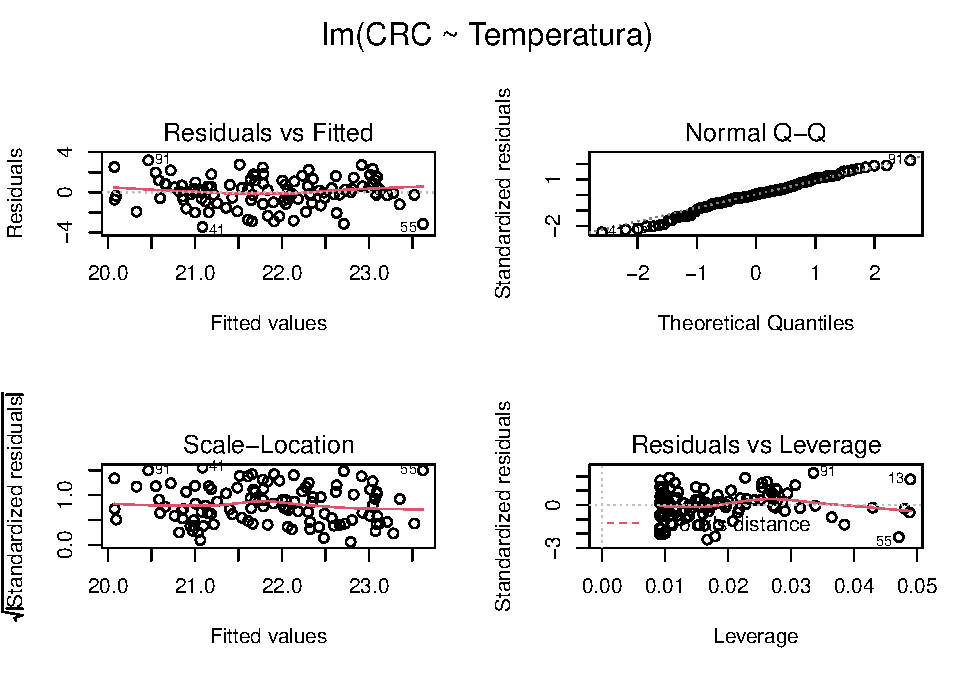
\includegraphics{livro_r_ecologia_files/figure-latex/unnamed-chunk-9-1.pdf}

\hypertarget{interpretauxe7uxe3o-dos-resultados-4}{%
\subsubsection{Interpretação dos resultados}\label{interpretauxe7uxe3o-dos-resultados-4}}

Com base no número de espécies raras (\emph{uniques} e \emph{duplicates}), Chao 2 estimou a possibilidade de encontrarmos mais dezesseis espécies caso o esforço amostral fosse maior e não mostrou tendência de estabilização da curva em uma assíntota.

\hypertarget{jackknife-1-burnham-overton-1978-1979}{%
\subsection{JACKKNIFE 1 (Burnham \& Overton 1978, 1979):}\label{jackknife-1-burnham-overton-1978-1979}}

Este estimador baseia-se no número de espécies que ocorrem em somente uma amostra (Q1).

\begin{quote}
\[S_{jack1} = S_{obs} + Q1\left(\frac{m - 1}{m}\right)\]
\end{quote}

onde:

\begin{itemize}
\item
  Sobs = o número de espécies na comunidade,
\item
  Q1 = número de espécies observadas em uma amostragem (espécies \emph{uniques}),
\item
  \emph{m} = número de amostragens.
\end{itemize}

Palmer (1990) verificou que Jackknife 1 foi o estimador mais preciso e menos enviesado comparado a outros métodos de extrapolação.

~

\hypertarget{exemplo-pruxe1tico---jackknife-1}{%
\subsubsection{Exemplo prático - Jackknife 1}\label{exemplo-pruxe1tico---jackknife-1}}

\hypertarget{explicauxe7uxe3o-dos-dados-3}{%
\paragraph{Explicação dos dados}\label{explicauxe7uxe3o-dos-dados-3}}

Usaremos os mesmos dados de 17 espécies de anuros amostradas em 14 dias de coletas de campo em um habitat reprodutivo localizado na região noroeste do estado de São Paulo, Brasil.

\textbf{Pergunta:}

\begin{quote}
Quantas espécies a mais poderiam ser amostradas caso aumentasse o esforço amostral?
\end{quote}

\textbf{Predições}

\begin{quote}
\begin{itemize}
\tightlist
\item
  O número de espécies estimadas é similar ao número de espécies observada;
\item
  O número de espécies estimadas é maior do que o número de espécies observada.
\end{itemize}
\end{quote}

\textbf{Variáveis}

\begin{itemize}
\tightlist
\item
  Variáveis preditoras

  \begin{itemize}
  \tightlist
  \item
    matriz ou vetor com as abundâncias das espécies de anuros registradas em uma habitat reprodutivo
  \end{itemize}
\end{itemize}

\textbf{Checklist}

\begin{itemize}
\tightlist
\item
  Verificar se a sua matriz está com as espécies nas colunas e as amostragens nas linhas
\end{itemize}

\hypertarget{anuxe1lise-5}{%
\subsection{Análise}\label{anuxe1lise-5}}

Calculo do estimador de riqueza - Jackknife 1

\begin{Shaded}
\begin{Highlighting}[]
\KeywordTok{library}\NormalTok{(vegan)}
\NormalTok{dados_coleta <-}\StringTok{ }\NormalTok{poca_anuros}
\NormalTok{est_jack1 <-}\StringTok{ }\KeywordTok{poolaccum}\NormalTok{(dados_coleta, }\DataTypeTok{permutations =} \DecValTok{100}\NormalTok{)}
\KeywordTok{summary}\NormalTok{(est_jack1, }\DataTypeTok{display =} \StringTok{"jack1"}\NormalTok{)}
\end{Highlighting}
\end{Shaded}

\begin{verbatim}
## $jack1
##        N Jackknife 1      2.5%    97.5%  Std.Dev
##  [1,]  3    14.15667  8.666667 21.00000 3.187537
##  [2,]  4    15.05000  9.750000 20.25000 2.908321
##  [3,]  5    15.87000 11.600000 20.70500 2.826766
##  [4,]  6    16.58333 11.229167 22.35000 2.901923
##  [5,]  7    17.51000 13.639286 23.85714 2.684791
##  [6,]  8    17.97875 13.290625 23.58437 2.631219
##  [7,]  9    18.96889 13.777778 24.11111 2.886258
##  [8,] 10    19.93600 14.747500 24.20000 2.630840
##  [9,] 11    20.53455 15.250000 24.27273 2.429309
## [10,] 12    21.36750 17.185417 23.89792 1.905751
## [11,] 13    21.85077 18.692308 23.46154 1.464411
## [12,] 14    22.57143 22.571429 22.57143 0.000000
## 
## attr(,"class")
## [1] "summary.poolaccum"
\end{verbatim}

Visualizar os resultados com 95\% intervalo de confiança

\begin{Shaded}
\begin{Highlighting}[]
\KeywordTok{library}\NormalTok{(ggplot2)}
\CommentTok{# preparando os dados para fazer o gráfico}
\NormalTok{resultados_jack1 <-}\StringTok{ }\KeywordTok{summary}\NormalTok{(est_jack1, }\DataTypeTok{display =} \KeywordTok{c}\NormalTok{(}\StringTok{"S"}\NormalTok{, }\StringTok{"jack1"}\NormalTok{))}
\NormalTok{res_jack1 <-}\StringTok{ }\KeywordTok{cbind}\NormalTok{(resultados_jack1}\OperatorTok{$}\NormalTok{jack1[,}\DecValTok{1}\OperatorTok{:}\DecValTok{4}\NormalTok{], resultados_jack1}\OperatorTok{$}\NormalTok{S[,}\DecValTok{2}\OperatorTok{:}\DecValTok{4}\NormalTok{])}
\NormalTok{res_jack1 <-}\StringTok{ }\KeywordTok{as.data.frame}\NormalTok{(res_jack1)}
\KeywordTok{colnames}\NormalTok{(res_jack1) <-}\StringTok{ }\KeywordTok{c}\NormalTok{(}\StringTok{"Amostras"}\NormalTok{, }\StringTok{"JACK1"}\NormalTok{, }\StringTok{"JACK1_inferior"}\NormalTok{, }\StringTok{"JACK1_superior"}\NormalTok{, }\StringTok{"Riqueza"}\NormalTok{,}
                        \StringTok{"R_inferior"}\NormalTok{, }\StringTok{"R_superior"}\NormalTok{)}

\CommentTok{# comando para o gráfico}
\KeywordTok{ggplot}\NormalTok{(res_jack1, }\KeywordTok{aes}\NormalTok{(}\DataTypeTok{y =}\NormalTok{ Riqueza, }\DataTypeTok{x =}\NormalTok{ Amostras)) }\OperatorTok{+}
\StringTok{  }\KeywordTok{geom_point}\NormalTok{(}\KeywordTok{aes}\NormalTok{(}\DataTypeTok{y =}\NormalTok{ JACK1, }\DataTypeTok{x =}\NormalTok{ Amostras }\OperatorTok{+}\StringTok{ }\FloatTok{0.1}\NormalTok{), }\DataTypeTok{size =} \DecValTok{5}\NormalTok{, }\DataTypeTok{color =} \StringTok{"blue"}\NormalTok{, }\DataTypeTok{alpha =} \DecValTok{1}\NormalTok{) }\OperatorTok{+}
\StringTok{  }\KeywordTok{geom_point}\NormalTok{(}\KeywordTok{aes}\NormalTok{(}\DataTypeTok{y =}\NormalTok{ Riqueza, }\DataTypeTok{x =}\NormalTok{ Amostras), }\DataTypeTok{size =} \DecValTok{5}\NormalTok{, }\DataTypeTok{color =} \StringTok{"red"}\NormalTok{, }\DataTypeTok{alpha =} \DecValTok{1}\NormalTok{) }\OperatorTok{+}
\StringTok{  }\KeywordTok{geom_line}\NormalTok{ (}\KeywordTok{aes}\NormalTok{(}\DataTypeTok{y =}\NormalTok{ JACK1, }\DataTypeTok{x =}\NormalTok{ Amostras), }\DataTypeTok{color =} \StringTok{"blue"}\NormalTok{) }\OperatorTok{+}
\StringTok{  }\KeywordTok{geom_line}\NormalTok{ (}\KeywordTok{aes}\NormalTok{(}\DataTypeTok{y =}\NormalTok{ Riqueza, }\DataTypeTok{x =}\NormalTok{ Amostras), }\DataTypeTok{color =} \StringTok{"red"}\NormalTok{) }\OperatorTok{+}
\StringTok{  }\KeywordTok{geom_linerange}\NormalTok{(}\KeywordTok{aes}\NormalTok{(}\DataTypeTok{ymin =}\NormalTok{ JACK1_inferior, }\DataTypeTok{ymax =}\NormalTok{ JACK1_superior, }\DataTypeTok{x =}\NormalTok{ Amostras }\OperatorTok{+}\StringTok{ }\FloatTok{0.1}\NormalTok{),}
 \DataTypeTok{color =} \StringTok{"blue"}\NormalTok{) }\OperatorTok{+}
\StringTok{  }\KeywordTok{geom_linerange}\NormalTok{(}\KeywordTok{aes}\NormalTok{(}\DataTypeTok{ymin =}\NormalTok{ R_inferior, }\DataTypeTok{ymax =}\NormalTok{ R_superior, }\DataTypeTok{x =}\NormalTok{ Amostras), }\DataTypeTok{color =} \StringTok{"red"}\NormalTok{) }\OperatorTok{+}
\StringTok{  }\KeywordTok{ylab}\NormalTok{ (}\StringTok{"Estimador de riqueza - Jackknife 1"}\NormalTok{) }\OperatorTok{+}
\StringTok{  }\KeywordTok{xlab}\NormalTok{ (}\StringTok{"Número de amostras"}\NormalTok{) }\OperatorTok{+}
\StringTok{  }\KeywordTok{scale_x_continuous}\NormalTok{(}\DataTypeTok{limits =} \KeywordTok{c}\NormalTok{(}\DecValTok{1}\NormalTok{,}\DecValTok{15}\NormalTok{), }\DataTypeTok{breaks=}\KeywordTok{seq}\NormalTok{(}\DecValTok{1}\NormalTok{,}\DecValTok{15}\NormalTok{,}\DecValTok{1}\NormalTok{)) }\OperatorTok{+}
\StringTok{  }\KeywordTok{geom_point}\NormalTok{(}\DataTypeTok{y=} \FloatTok{9.9}\NormalTok{, }\DataTypeTok{x =} \DecValTok{9}\NormalTok{, }\DataTypeTok{size =} \DecValTok{5}\NormalTok{, }\DataTypeTok{color =} \StringTok{"blue"}\NormalTok{, }\DataTypeTok{alpha =} \DecValTok{1}\NormalTok{) }\OperatorTok{+}\StringTok{ }
\StringTok{  }\KeywordTok{geom_point}\NormalTok{(}\DataTypeTok{y=} \FloatTok{8.6}\NormalTok{, }\DataTypeTok{x =} \DecValTok{9}\NormalTok{, }\DataTypeTok{size =} \DecValTok{5}\NormalTok{, }\DataTypeTok{color =} \StringTok{"red"}\NormalTok{, }\DataTypeTok{alpha =} \DecValTok{1}\NormalTok{) }\OperatorTok{+}\StringTok{ }
\StringTok{  }\KeywordTok{geom_label}\NormalTok{( }\DataTypeTok{y =} \FloatTok{9.9}\NormalTok{, }\DataTypeTok{x =} \FloatTok{12.5}\NormalTok{, }\DataTypeTok{label =} \StringTok{"Riqueza estimada - Jackknife 1"}\NormalTok{) }\OperatorTok{+}
\StringTok{  }\KeywordTok{geom_label}\NormalTok{( }\DataTypeTok{y =} \FloatTok{8.6}\NormalTok{, }\DataTypeTok{x =} \FloatTok{11.5}\NormalTok{, }\DataTypeTok{label =} \StringTok{"Riqueza observada"}\NormalTok{)}
\end{Highlighting}
\end{Shaded}

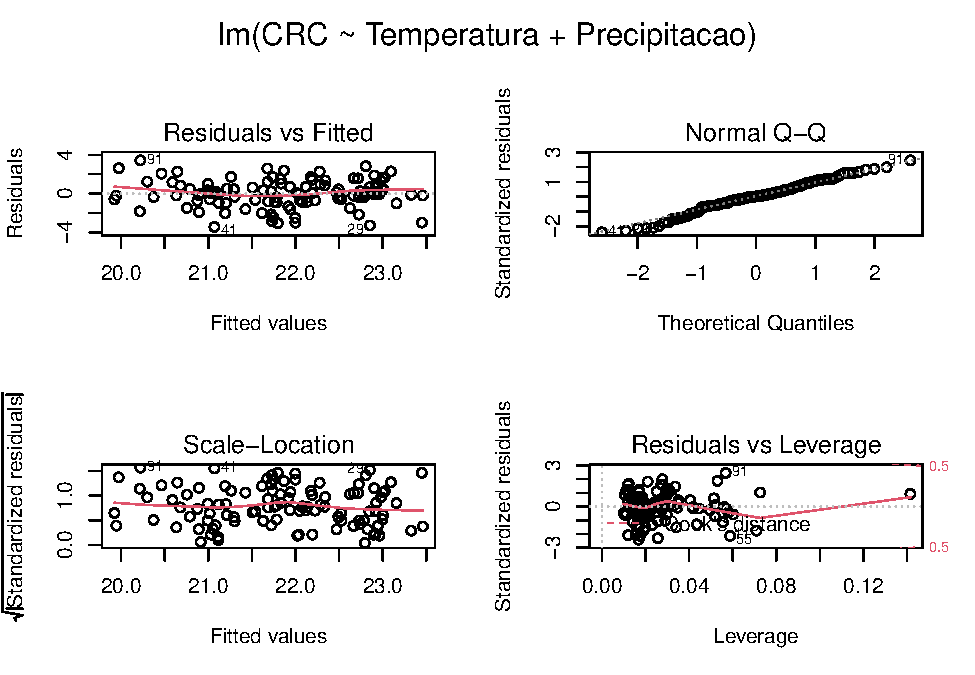
\includegraphics{livro_r_ecologia_files/figure-latex/unnamed-chunk-11-1.pdf}

\hypertarget{interpretauxe7uxe3o-dos-resultados-5}{%
\subsubsection{Interpretação dos resultados}\label{interpretauxe7uxe3o-dos-resultados-5}}

Com base no número de espécies raras, o estimador Jackknife 1 calculou a possibilidade de encontrarmos mais seis espécies caso o esforço amostral fosse maior e não mostrou tendência de estabilização da curva em uma assíntota.

\hypertarget{jackknife-2-burnham-overton-1978-1979-palmer-1991}{%
\subsection{JACKKNIFE 2 (Burnham \& Overton 1978, 1979, Palmer 1991):}\label{jackknife-2-burnham-overton-1978-1979-palmer-1991}}

Este método basea-se no número de espécies que ocorrem em apenas uma amostra e no número de espécies que ocorrem em exatamente duas amostras.

\begin{quote}
\[S_{jack2} = S_{obs} + \left[\frac{Q_1(2m - 3)}{m}-\frac{Q_2(m - 2)^2}{m(m-1)}\right]\]
\end{quote}

onde:

\begin{itemize}
\item
  Sobs = o número de espécies na comunidade,
\item
  \emph{m} = número de amostragens,
\item
  Q1 = número de espécies observadas em uma amostragem (espécies \emph{uniques}),
\item
  Q2 = número de espécies observadas em duas amostragens (espécies \emph{duplicates}).
\end{itemize}

~

\hypertarget{exemplo-pruxe1tico---jackknife-2}{%
\subsubsection{Exemplo prático - Jackknife 2}\label{exemplo-pruxe1tico---jackknife-2}}

\hypertarget{explicauxe7uxe3o-dos-dados-4}{%
\paragraph{Explicação dos dados}\label{explicauxe7uxe3o-dos-dados-4}}

Usaremos os mesmos dados de 17 espécies de anuros amostradas em 14 dias de coletas de campo em um habitat reprodutivo localizado na região noroeste do estado de São Paulo, Brasil.

\textbf{Pergunta:}

\begin{quote}
Quantas espécies a mais poderiam ser amostradas caso aumentasse o esforço amostral?
\end{quote}

\textbf{Predições}

\begin{quote}
\begin{itemize}
\tightlist
\item
  O número de espécies estimadas é similar ao número de espécies observada;
\item
  O número de espécies estimadas é maior do que o número de espécies observada.
\end{itemize}
\end{quote}

\textbf{Variáveis}

\begin{itemize}
\tightlist
\item
  Variáveis preditoras

  \begin{itemize}
  \tightlist
  \item
    matriz ou vetor com as abundâncias das espécies de anuros registradas em uma habitat reprodutivo
  \end{itemize}
\end{itemize}

\textbf{Checklist}

\begin{itemize}
\tightlist
\item
  Verificar se a sua matriz está com as espécies nas colunas e as amostragens nas linhas
\end{itemize}

\hypertarget{anuxe1lise-6}{%
\subsection{Análise}\label{anuxe1lise-6}}

Calculo do estimador de riqueza - Jackknife 2

\begin{Shaded}
\begin{Highlighting}[]
\KeywordTok{library}\NormalTok{(vegan)}
\NormalTok{dados_coleta <-}\StringTok{ }\NormalTok{poca_anuros}
\NormalTok{est_jack2 <-}\StringTok{ }\KeywordTok{poolaccum}\NormalTok{(dados_coleta, }\DataTypeTok{permutations =} \DecValTok{100}\NormalTok{)}
\KeywordTok{summary}\NormalTok{(est_jack2, }\DataTypeTok{display =} \StringTok{"jack2"}\NormalTok{)}
\end{Highlighting}
\end{Shaded}

\begin{verbatim}
## $jack2
##        N Jackknife 2      2.5%    97.5%  Std.Dev
##  [1,]  3    15.04167  7.666667 21.58750 3.445534
##  [2,]  4    15.49250  8.866667 23.04375 3.688470
##  [3,]  5    16.81950  9.293750 24.40250 3.661352
##  [4,]  6    18.15233 10.153333 25.96667 4.144035
##  [5,]  7    19.51214 12.952381 26.12202 4.030475
##  [6,]  8    20.78768 13.776786 29.35714 4.230203
##  [7,]  9    21.81639 14.485069 29.21840 4.114662
##  [8,] 10    23.06389 14.977778 29.45472 3.759535
##  [9,] 11    24.18464 15.718182 28.35455 3.418031
## [10,] 12    24.97659 19.323674 28.49242 2.715636
## [11,] 13    26.14160 21.301282 28.60897 1.738847
## [12,] 14    26.92308 26.923077 26.92308 0.000000
## 
## attr(,"class")
## [1] "summary.poolaccum"
\end{verbatim}

Visualizar os resultados com intervalo de confiança de 95\%

\begin{Shaded}
\begin{Highlighting}[]
\KeywordTok{library}\NormalTok{(ggplot2)}
\CommentTok{# preparando os dados para fazer o gráfico}
\NormalTok{resultados_jack2 <-}\StringTok{ }\KeywordTok{summary}\NormalTok{(est_jack2, }\DataTypeTok{display =} \KeywordTok{c}\NormalTok{(}\StringTok{"S"}\NormalTok{, }\StringTok{"jack2"}\NormalTok{))}
\NormalTok{res_jack2 <-}\StringTok{ }\KeywordTok{cbind}\NormalTok{(resultados_jack2}\OperatorTok{$}\NormalTok{jack2[,}\DecValTok{1}\OperatorTok{:}\DecValTok{4}\NormalTok{], resultados_jack2}\OperatorTok{$}\NormalTok{S[,}\DecValTok{2}\OperatorTok{:}\DecValTok{4}\NormalTok{])}
\NormalTok{res_jack2 <-}\StringTok{ }\KeywordTok{as.data.frame}\NormalTok{(res_jack2)}
\KeywordTok{colnames}\NormalTok{(res_jack2) <-}\StringTok{ }\KeywordTok{c}\NormalTok{(}\StringTok{"Amostras"}\NormalTok{, }\StringTok{"JACK2"}\NormalTok{, }\StringTok{"JACK2_inferior"}\NormalTok{, }\StringTok{"JACK2_superior"}\NormalTok{, }\StringTok{"Riqueza"}\NormalTok{,}
                        \StringTok{"R_inferior"}\NormalTok{, }\StringTok{"R_superior"}\NormalTok{)}

\CommentTok{# comando para o gráfico}
\KeywordTok{ggplot}\NormalTok{(res_jack2, }\KeywordTok{aes}\NormalTok{(}\DataTypeTok{y =}\NormalTok{ Riqueza, }\DataTypeTok{x =}\NormalTok{ Amostras)) }\OperatorTok{+}
\StringTok{  }\KeywordTok{geom_point}\NormalTok{(}\KeywordTok{aes}\NormalTok{(}\DataTypeTok{y =}\NormalTok{ JACK2, }\DataTypeTok{x =}\NormalTok{ Amostras }\OperatorTok{+}\StringTok{ }\FloatTok{0.1}\NormalTok{), }\DataTypeTok{size =} \DecValTok{5}\NormalTok{, }\DataTypeTok{color =} \StringTok{"blue"}\NormalTok{, }\DataTypeTok{alpha =} \DecValTok{1}\NormalTok{) }\OperatorTok{+}
\StringTok{  }\KeywordTok{geom_point}\NormalTok{(}\KeywordTok{aes}\NormalTok{(}\DataTypeTok{y =}\NormalTok{ Riqueza, }\DataTypeTok{x =}\NormalTok{ Amostras), }\DataTypeTok{size =} \DecValTok{5}\NormalTok{, }\DataTypeTok{color =} \StringTok{"red"}\NormalTok{, }\DataTypeTok{alpha =} \DecValTok{1}\NormalTok{) }\OperatorTok{+}
\StringTok{  }\KeywordTok{geom_line}\NormalTok{ (}\KeywordTok{aes}\NormalTok{(}\DataTypeTok{y =}\NormalTok{ JACK2, }\DataTypeTok{x =}\NormalTok{ Amostras), }\DataTypeTok{color =} \StringTok{"blue"}\NormalTok{) }\OperatorTok{+}
\StringTok{  }\KeywordTok{geom_line}\NormalTok{ (}\KeywordTok{aes}\NormalTok{(}\DataTypeTok{y =}\NormalTok{ Riqueza, }\DataTypeTok{x =}\NormalTok{ Amostras), }\DataTypeTok{color =} \StringTok{"red"}\NormalTok{) }\OperatorTok{+}
\StringTok{  }\KeywordTok{geom_linerange}\NormalTok{(}\KeywordTok{aes}\NormalTok{(}\DataTypeTok{ymin =}\NormalTok{ JACK2_inferior, }\DataTypeTok{ymax =}\NormalTok{ JACK2_superior, }\DataTypeTok{x =}\NormalTok{ Amostras }\OperatorTok{+}\StringTok{ }\FloatTok{0.1}\NormalTok{),}
 \DataTypeTok{color =} \StringTok{"blue"}\NormalTok{) }\OperatorTok{+}
\StringTok{  }\KeywordTok{geom_linerange}\NormalTok{(}\KeywordTok{aes}\NormalTok{(}\DataTypeTok{ymin =}\NormalTok{ R_inferior, }\DataTypeTok{ymax =}\NormalTok{ R_superior, }\DataTypeTok{x =}\NormalTok{ Amostras), }\DataTypeTok{color =} \StringTok{"red"}\NormalTok{) }\OperatorTok{+}
\StringTok{  }\KeywordTok{ylab}\NormalTok{ (}\StringTok{"Estimador de riqueza - Jackknife 2"}\NormalTok{) }\OperatorTok{+}
\StringTok{  }\KeywordTok{xlab}\NormalTok{ (}\StringTok{"Número de amostras"}\NormalTok{) }\OperatorTok{+}
\StringTok{  }\KeywordTok{scale_x_continuous}\NormalTok{(}\DataTypeTok{limits =} \KeywordTok{c}\NormalTok{(}\DecValTok{1}\NormalTok{,}\DecValTok{15}\NormalTok{), }\DataTypeTok{breaks=}\KeywordTok{seq}\NormalTok{(}\DecValTok{1}\NormalTok{,}\DecValTok{15}\NormalTok{,}\DecValTok{1}\NormalTok{)) }\OperatorTok{+}
\StringTok{  }\KeywordTok{geom_point}\NormalTok{(}\DataTypeTok{y=} \FloatTok{9.9}\NormalTok{, }\DataTypeTok{x =} \DecValTok{9}\NormalTok{, }\DataTypeTok{size =} \DecValTok{5}\NormalTok{, }\DataTypeTok{color =} \StringTok{"blue"}\NormalTok{, }\DataTypeTok{alpha =} \DecValTok{1}\NormalTok{) }\OperatorTok{+}\StringTok{ }
\StringTok{  }\KeywordTok{geom_point}\NormalTok{(}\DataTypeTok{y=} \FloatTok{8.2}\NormalTok{, }\DataTypeTok{x =} \DecValTok{9}\NormalTok{, }\DataTypeTok{size =} \DecValTok{5}\NormalTok{, }\DataTypeTok{color =} \StringTok{"red"}\NormalTok{, }\DataTypeTok{alpha =} \DecValTok{1}\NormalTok{) }\OperatorTok{+}\StringTok{ }
\StringTok{  }\KeywordTok{geom_label}\NormalTok{( }\DataTypeTok{y =} \FloatTok{9.9}\NormalTok{, }\DataTypeTok{x =} \FloatTok{12.5}\NormalTok{, }\DataTypeTok{label =} \StringTok{"Riqueza estimada - Jackknife 2"}\NormalTok{) }\OperatorTok{+}
\StringTok{  }\KeywordTok{geom_label}\NormalTok{( }\DataTypeTok{y =} \FloatTok{8.2}\NormalTok{, }\DataTypeTok{x =} \FloatTok{11.5}\NormalTok{, }\DataTypeTok{label =} \StringTok{"Riqueza observada"}\NormalTok{)}
\end{Highlighting}
\end{Shaded}

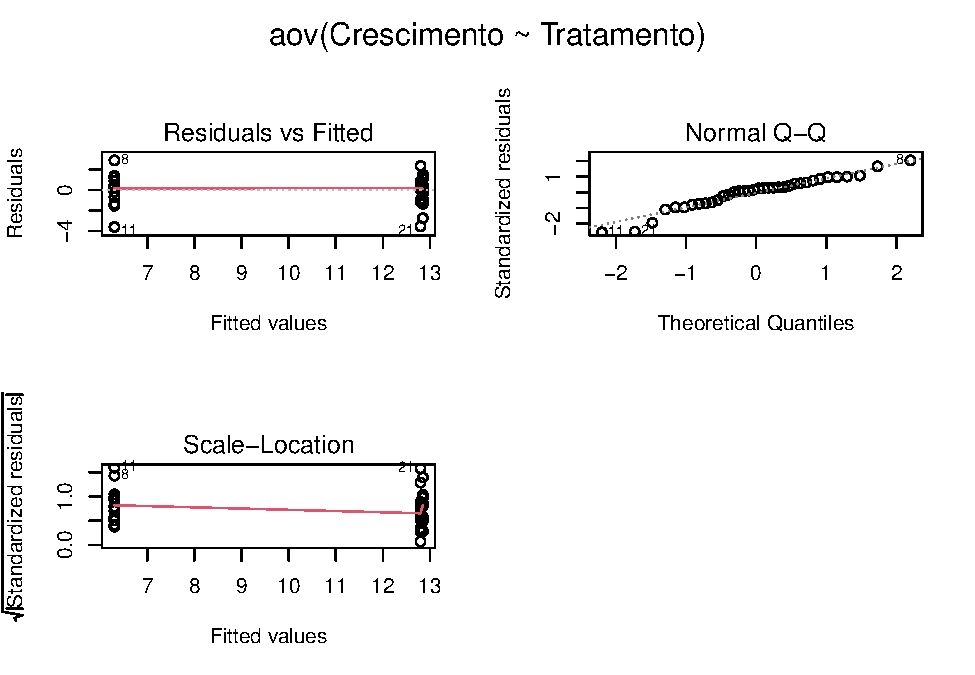
\includegraphics{livro_r_ecologia_files/figure-latex/unnamed-chunk-13-1.pdf}

\hypertarget{interpretauxe7uxe3o-dos-resultados-6}{%
\subsubsection{Interpretação dos resultados}\label{interpretauxe7uxe3o-dos-resultados-6}}

Com base no número de espécies raras, o estimador Jackknife 2 calculou a possibilidade de encontrarmos mais dez espécies caso o esforço amostral fosse maior e não mostrou tendência estabilização da curva em uma assíntota.

\hypertarget{bootstrap-smith-van-belle-1984}{%
\subsection{BOOTSTRAP (Smith \& van Belle 1984):}\label{bootstrap-smith-van-belle-1984}}

Este método difere dos demais por utilizar dados de todas as espécies coletadas para estimar a riqueza total, não se restringindo às espécies raras. Ele requer somente dados de incidência. A estimativa pelo bootstrap é calculada somando-se a riqueza observada à soma do inverso da proporção de amostras em que cada espécie ocorre.

\begin{quote}
\[S_{boot} = S_{obs} + \sum_{k=1}^{S_{obs}}(1-P_k)^m\]
\end{quote}

onde:

\begin{itemize}
\item
  Sobs = o número de espécies na comunidade,
\item
  \emph{m} = número de amostragens,
\item
  Pk = proporção do número de amostras em que cada espécie foi registrada.
\end{itemize}

~

\hypertarget{exemplo-pruxe1tico---bootstrap}{%
\subsubsection{Exemplo prático - Bootstrap}\label{exemplo-pruxe1tico---bootstrap}}

\hypertarget{explicauxe7uxe3o-dos-dados-5}{%
\paragraph{Explicação dos dados}\label{explicauxe7uxe3o-dos-dados-5}}

Usaremos os mesmos dados de 17 espécies de anuros amostradas em 14 dias de coletas de campo em um habitat reprodutivo localizado na região noroeste do estado de São Paulo, Brasil.

\textbf{Pergunta:}

\begin{quote}
Quantas espécies a mais poderiam ser amostradas caso aumentasse o esforço amostral?
\end{quote}

\textbf{Predições}

\begin{quote}
\begin{itemize}
\tightlist
\item
  O número de espécies estimadas é similar ao número de espécies observada;
\item
  O número de espécies estimadas é maior do que o número de espécies observada.
\end{itemize}
\end{quote}

\textbf{Variáveis}

\begin{itemize}
\tightlist
\item
  Variáveis preditoras

  \begin{itemize}
  \tightlist
  \item
    matriz ou vetor com as abundâncias das espécies de anuros registradas em uma habitat reprodutivo
  \end{itemize}
\end{itemize}

\textbf{Checklist}

\begin{itemize}
\tightlist
\item
  Verificar se a sua matriz está com as espécies nas colunas e as amostragens nas linhas
\end{itemize}

\hypertarget{anuxe1lise-7}{%
\subsection{Análise}\label{anuxe1lise-7}}

Calculo do estimador de riqueza - Bootstrap

\begin{Shaded}
\begin{Highlighting}[]
\KeywordTok{library}\NormalTok{(vegan)}
\NormalTok{dados_coleta <-}\StringTok{ }\NormalTok{poca_anuros}
\NormalTok{est_boot <-}\StringTok{ }\KeywordTok{poolaccum}\NormalTok{(dados_coleta, }\DataTypeTok{permutations =} \DecValTok{100}\NormalTok{)}
\KeywordTok{summary}\NormalTok{(est_boot, }\DataTypeTok{display =} \StringTok{"boot"}\NormalTok{)}
\end{Highlighting}
\end{Shaded}

\begin{verbatim}
## $boot
##        N Bootstrap      2.5%    97.5%   Std.Dev
##  [1,]  3  11.47778  7.517593 16.16759 2.2218138
##  [2,]  4  12.53539  8.457031 16.22490 2.2228959
##  [3,]  5  13.59872  9.701288 17.39817 1.9848709
##  [4,]  6  14.39329 11.172274 17.91056 1.7777948
##  [5,]  7  15.15844 11.820110 18.96258 1.8767058
##  [6,]  8  15.91556 12.766099 19.29035 1.8632981
##  [7,]  9  16.40730 13.006320 19.45435 1.7932676
##  [8,] 10  17.06085 13.011781 19.80358 1.8958075
##  [9,] 11  17.64928 13.929216 19.81378 1.7133537
## [10,] 12  18.26775 15.233580 19.82092 1.3823778
## [11,] 13  18.73539 16.570376 19.59107 0.9919236
## [12,] 14  19.27832 19.278321 19.27832 0.0000000
## 
## attr(,"class")
## [1] "summary.poolaccum"
\end{verbatim}

Visualizar os resultados com intervalo de confiança de 95\%

\begin{Shaded}
\begin{Highlighting}[]
\KeywordTok{library}\NormalTok{(ggplot2)}
\CommentTok{# preparando os dados para fazer o gráfico}
\NormalTok{resultados_boot <-}\StringTok{ }\KeywordTok{summary}\NormalTok{(est_boot, }\DataTypeTok{display =} \KeywordTok{c}\NormalTok{(}\StringTok{"S"}\NormalTok{, }\StringTok{"boot"}\NormalTok{))}
\NormalTok{res_boot <-}\StringTok{ }\KeywordTok{cbind}\NormalTok{(resultados_boot}\OperatorTok{$}\NormalTok{boot[,}\DecValTok{1}\OperatorTok{:}\DecValTok{4}\NormalTok{], resultados_boot}\OperatorTok{$}\NormalTok{S[,}\DecValTok{2}\OperatorTok{:}\DecValTok{4}\NormalTok{])}
\NormalTok{res_boot <-}\StringTok{ }\KeywordTok{as.data.frame}\NormalTok{(res_boot)}
\KeywordTok{colnames}\NormalTok{(res_boot) <-}\StringTok{ }\KeywordTok{c}\NormalTok{(}\StringTok{"Amostras"}\NormalTok{, }\StringTok{"BOOT"}\NormalTok{, }\StringTok{"BOOT_inferior"}\NormalTok{, }\StringTok{"BOOT_superior"}\NormalTok{, }\StringTok{"Riqueza"}\NormalTok{,}
                        \StringTok{"R_inferior"}\NormalTok{, }\StringTok{"R_superior"}\NormalTok{)}

\CommentTok{# comando para o gráfico}
\KeywordTok{ggplot}\NormalTok{(res_boot, }\KeywordTok{aes}\NormalTok{(}\DataTypeTok{y =}\NormalTok{ Riqueza, }\DataTypeTok{x =}\NormalTok{ Amostras)) }\OperatorTok{+}
\StringTok{  }\KeywordTok{geom_point}\NormalTok{(}\KeywordTok{aes}\NormalTok{(}\DataTypeTok{y =}\NormalTok{ BOOT, }\DataTypeTok{x =}\NormalTok{ Amostras }\OperatorTok{+}\StringTok{ }\FloatTok{0.1}\NormalTok{), }\DataTypeTok{size =} \DecValTok{5}\NormalTok{, }\DataTypeTok{color =} \StringTok{"blue"}\NormalTok{, }\DataTypeTok{alpha =} \DecValTok{1}\NormalTok{) }\OperatorTok{+}
\StringTok{  }\KeywordTok{geom_point}\NormalTok{(}\KeywordTok{aes}\NormalTok{(}\DataTypeTok{y =}\NormalTok{ Riqueza, }\DataTypeTok{x =}\NormalTok{ Amostras), }\DataTypeTok{size =} \DecValTok{5}\NormalTok{, }\DataTypeTok{color =} \StringTok{"red"}\NormalTok{, }\DataTypeTok{alpha =} \DecValTok{1}\NormalTok{) }\OperatorTok{+}
\StringTok{  }\KeywordTok{geom_line}\NormalTok{ (}\KeywordTok{aes}\NormalTok{(}\DataTypeTok{y =}\NormalTok{ BOOT, }\DataTypeTok{x =}\NormalTok{ Amostras), }\DataTypeTok{color =} \StringTok{"blue"}\NormalTok{) }\OperatorTok{+}
\StringTok{  }\KeywordTok{geom_line}\NormalTok{ (}\KeywordTok{aes}\NormalTok{(}\DataTypeTok{y =}\NormalTok{ Riqueza, }\DataTypeTok{x =}\NormalTok{ Amostras), }\DataTypeTok{color =} \StringTok{"red"}\NormalTok{) }\OperatorTok{+}
\StringTok{  }\KeywordTok{geom_linerange}\NormalTok{(}\KeywordTok{aes}\NormalTok{(}\DataTypeTok{ymin =}\NormalTok{ BOOT_inferior, }\DataTypeTok{ymax =}\NormalTok{ BOOT_superior, }\DataTypeTok{x =}\NormalTok{ Amostras }\OperatorTok{+}\StringTok{ }\FloatTok{0.1}\NormalTok{),}
 \DataTypeTok{color =} \StringTok{"blue"}\NormalTok{) }\OperatorTok{+}
\StringTok{  }\KeywordTok{geom_linerange}\NormalTok{(}\KeywordTok{aes}\NormalTok{(}\DataTypeTok{ymin =}\NormalTok{ R_inferior, }\DataTypeTok{ymax =}\NormalTok{ R_superior, }\DataTypeTok{x =}\NormalTok{ Amostras), }\DataTypeTok{color =} \StringTok{"red"}\NormalTok{) }\OperatorTok{+}
\StringTok{  }\KeywordTok{ylab}\NormalTok{ (}\StringTok{"Estimador de riqueza - Bootstrap"}\NormalTok{) }\OperatorTok{+}
\StringTok{  }\KeywordTok{xlab}\NormalTok{ (}\StringTok{"Número de amostras"}\NormalTok{) }\OperatorTok{+}
\StringTok{  }\KeywordTok{scale_x_continuous}\NormalTok{(}\DataTypeTok{limits =} \KeywordTok{c}\NormalTok{(}\DecValTok{1}\NormalTok{,}\DecValTok{15}\NormalTok{), }\DataTypeTok{breaks=}\KeywordTok{seq}\NormalTok{(}\DecValTok{1}\NormalTok{,}\DecValTok{15}\NormalTok{,}\DecValTok{1}\NormalTok{)) }\OperatorTok{+}
\StringTok{  }\KeywordTok{geom_point}\NormalTok{(}\DataTypeTok{y=} \FloatTok{10.4}\NormalTok{, }\DataTypeTok{x =} \FloatTok{9.5}\NormalTok{, }\DataTypeTok{size =} \DecValTok{5}\NormalTok{, }\DataTypeTok{color =} \StringTok{"blue"}\NormalTok{, }\DataTypeTok{alpha =} \DecValTok{1}\NormalTok{) }\OperatorTok{+}\StringTok{ }
\StringTok{  }\KeywordTok{geom_point}\NormalTok{(}\DataTypeTok{y=} \FloatTok{9.3}\NormalTok{, }\DataTypeTok{x =} \FloatTok{9.5}\NormalTok{, }\DataTypeTok{size =} \DecValTok{5}\NormalTok{, }\DataTypeTok{color =} \StringTok{"red"}\NormalTok{, }\DataTypeTok{alpha =} \DecValTok{1}\NormalTok{) }\OperatorTok{+}\StringTok{ }
\StringTok{  }\KeywordTok{geom_label}\NormalTok{( }\DataTypeTok{y =} \FloatTok{10.4}\NormalTok{, }\DataTypeTok{x =} \FloatTok{12.3}\NormalTok{, }\DataTypeTok{label =} \StringTok{"Riqueza estimada - Bootstrap"}\NormalTok{) }\OperatorTok{+}
\StringTok{  }\KeywordTok{geom_label}\NormalTok{( }\DataTypeTok{y =} \FloatTok{9.3}\NormalTok{, }\DataTypeTok{x =} \FloatTok{11.5}\NormalTok{, }\DataTypeTok{label =} \StringTok{"Riqueza observada"}\NormalTok{)}
\end{Highlighting}
\end{Shaded}

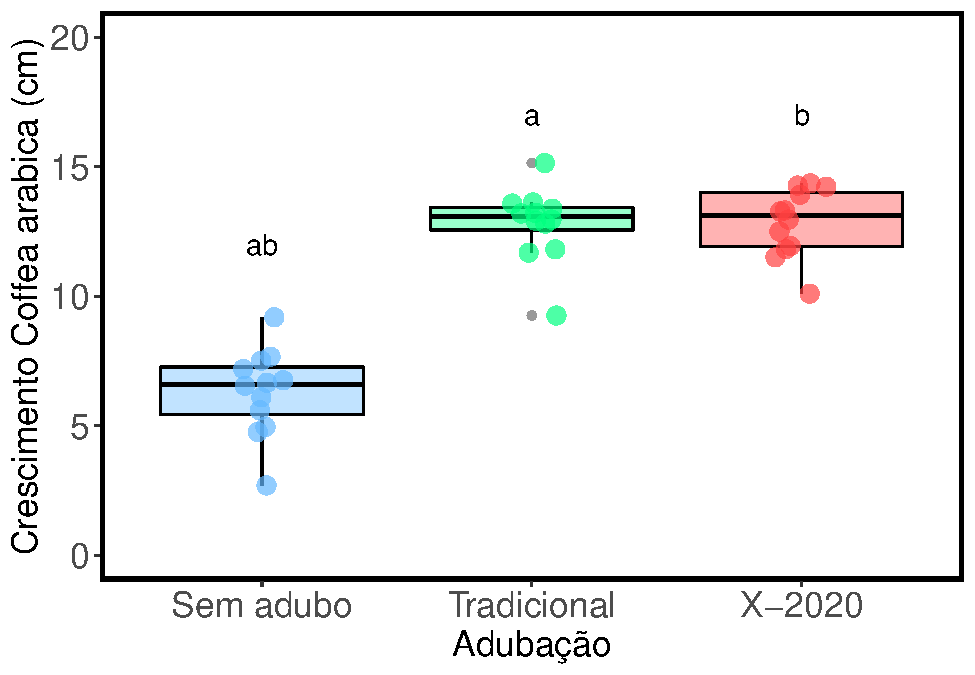
\includegraphics{livro_r_ecologia_files/figure-latex/unnamed-chunk-15-1.pdf}

\hypertarget{interpretauxe7uxe3o-dos-resultados-7}{%
\subsubsection{Interpretação dos resultados}\label{interpretauxe7uxe3o-dos-resultados-7}}

Com base na frequencia de ocorrência das espécies, o estimador bootstrap calculou a possibilidade de encontrarmos mais duas espécies caso o esforço amostral fosse maior e não mostrou tendência de estabilização da curva em uma assíntota.

\hypertarget{interpolauxe7uxe3o-e-extrapolauxe7uxe3o-baseadas-em-rarefauxe7uxe3o-usando-amostragens-de-inciduxeancia-ou-abunduxe2ncia-chao-jost-2012-colwell-et-al.-2012}{%
\subsection{Interpolação e Extrapolação baseadas em rarefação usando amostragens de incidência ou abundância (Chao \& Jost 2012, Colwell et al.~2012):}\label{interpolauxe7uxe3o-e-extrapolauxe7uxe3o-baseadas-em-rarefauxe7uxe3o-usando-amostragens-de-inciduxeancia-ou-abunduxe2ncia-chao-jost-2012-colwell-et-al.-2012}}

Este método utiliza teoria de amostragem (e.g.~modelos multinomial, Poisson e Bernoulli) para conectar rarefação (interpolação) e predição (extrapolação) com base no tamanho da amostra. Contudo, é importante enfatizar que a extrapolação torna-se altamente incerta quando extendida para o dobro do tamanho da amostragem. Este método utiliza uma abordagem com bootstrap para calcular o intervalo de confiança de 95\%.

\hypertarget{exemplo-pruxe1tico}{%
\subsubsection{Exemplo prático}\label{exemplo-pruxe1tico}}

\hypertarget{explicauxe7uxe3o-dos-dados-6}{%
\paragraph{Explicação dos dados}\label{explicauxe7uxe3o-dos-dados-6}}

Usaremos os mesmos dados de 17 espécies de anuros amostradas em 14 dias de coletas de campo em um habitat reprodutivo localizado na região noroeste do estado de São Paulo, Brasil.

\textbf{Pergunta:}

\begin{quote}
Quantas espécies a mais poderiam ser amostradas caso aumentasse o esforço amostral?
\end{quote}

\textbf{Predições}

\begin{quote}
\begin{itemize}
\tightlist
\item
  O número de espécies estimadas é similar ao número de espécies observada;
\item
  O número de espécies estimadas é maior do que o número de espécies observada.
\end{itemize}
\end{quote}

\textbf{Variáveis}

\begin{itemize}
\tightlist
\item
  Variáveis preditoras

  \begin{itemize}
  \tightlist
  \item
    matriz ou vetor com as abundâncias das espécies de anuros registradas em uma habitat reprodutivo
  \end{itemize}
\end{itemize}

\textbf{Checklist}

\begin{itemize}
\tightlist
\item
  Verificar se a sua matriz está com as espécies nas colunas e as amostragens nas linhas.
\end{itemize}

\hypertarget{anuxe1lise-8}{%
\subsection{Análise}\label{anuxe1lise-8}}

Calculo da extrapolação da riqueza com base no número de indivíduos

\begin{Shaded}
\begin{Highlighting}[]
\KeywordTok{library}\NormalTok{(iNEXT)}
\NormalTok{dados_coleta <-}\StringTok{ }\NormalTok{poca_anuros}

\CommentTok{# preparando os dados para análises considerando a abundância}
\NormalTok{dados_inext_abu <-}\StringTok{ }\KeywordTok{colSums}\NormalTok{(dados_coleta) }

\NormalTok{resultados_abundancia <-}\StringTok{ }\KeywordTok{iNEXT}\NormalTok{(dados_inext_abu, }\DataTypeTok{q =} \DecValTok{0}\NormalTok{, }\DataTypeTok{datatype =} \StringTok{"abundance"}\NormalTok{, }
            \DataTypeTok{endpoint =} \DecValTok{600}\NormalTok{)}

\CommentTok{# Visualizar os dados no gráfico}
\KeywordTok{ggiNEXT}\NormalTok{(resultados_abundancia, }\DataTypeTok{type =} \DecValTok{1}\NormalTok{)}
\end{Highlighting}
\end{Shaded}

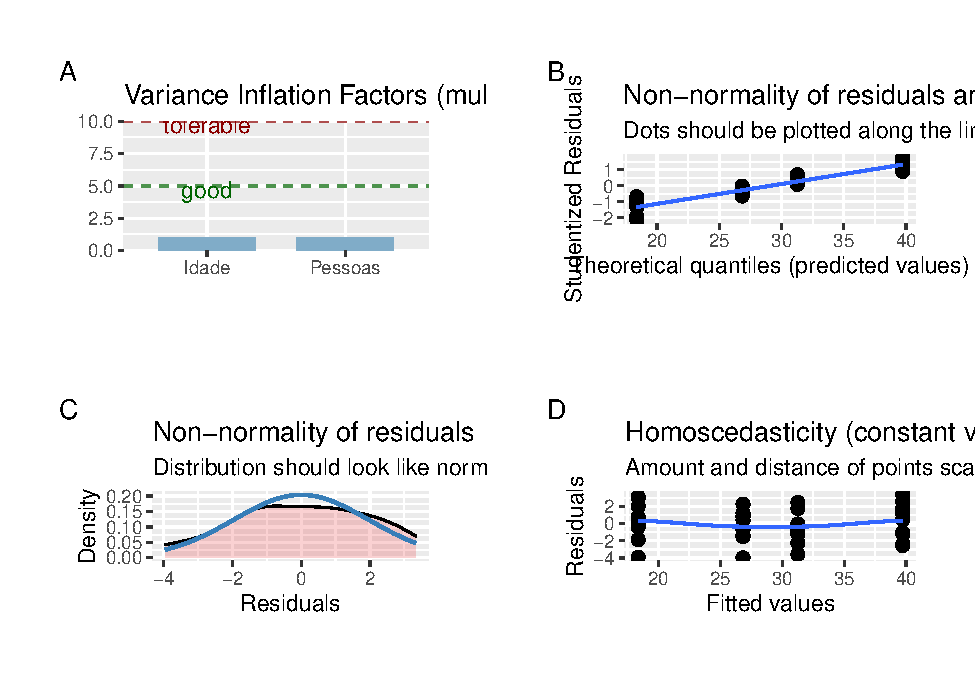
\includegraphics{livro_r_ecologia_files/figure-latex/unnamed-chunk-16-1.pdf}

\hypertarget{interpretauxe7uxe3o-dos-resultados-8}{%
\subsubsection{Interpretação dos resultados}\label{interpretauxe7uxe3o-dos-resultados-8}}

Veja que o ponto no final da linha contínua representa as 17 espécies de anuros (eixo Y) observadas entre os 304 individuos (eixo X). A extrapolação máxima (600 indivíduos no nosso exemplo), estima um aumento de até oito espécies (intervalo de confiança) caso amostrássemos mais 300 indivíduos.

Calculo da extrapolação da riqueza com base no número de amostras

\begin{Shaded}
\begin{Highlighting}[]
\KeywordTok{library}\NormalTok{(iNEXT)}
\NormalTok{dados_coleta <-}\StringTok{ }\NormalTok{poca_anuros}

\CommentTok{# preparando os dados para análises considerando a incidência}
\NormalTok{dados_inext <-}\StringTok{ }\KeywordTok{as.incfreq}\NormalTok{(}\KeywordTok{t}\NormalTok{(dados_coleta)) }\CommentTok{# preciso transpor o dataframe}

\NormalTok{resultados_incidencia <-}\StringTok{ }\KeywordTok{iNEXT}\NormalTok{(dados_inext, }\DataTypeTok{q =} \DecValTok{0}\NormalTok{, }\DataTypeTok{datatype =} \StringTok{"incidence_freq"}\NormalTok{, }
            \DataTypeTok{endpoint =} \DecValTok{30}\NormalTok{)}

\CommentTok{# Visualizar os dados no gráfico}
\KeywordTok{ggiNEXT}\NormalTok{(resultados_incidencia, }\DataTypeTok{type =} \DecValTok{1}\NormalTok{)}
\end{Highlighting}
\end{Shaded}

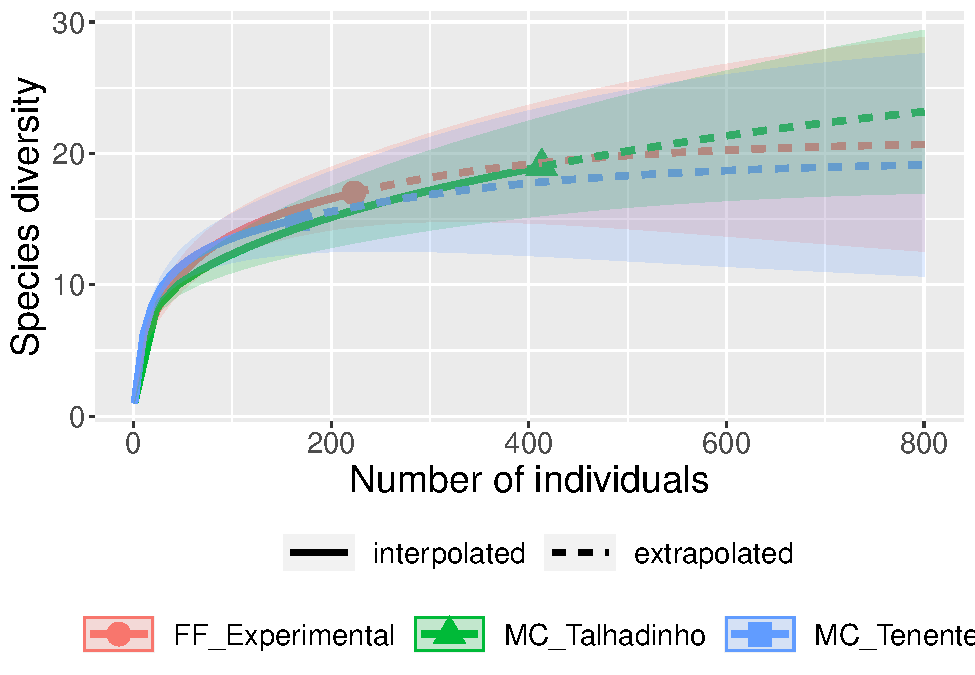
\includegraphics{livro_r_ecologia_files/figure-latex/unnamed-chunk-17-1.pdf}

\hypertarget{interpretauxe7uxe3o-dos-resultados-9}{%
\subsubsection{Interpretação dos resultados}\label{interpretauxe7uxe3o-dos-resultados-9}}

Veja que o ponto no final da linha contínua representa as 17 espécies de anuros (eixo Y) observadas nos 14 dias de coleta (eixo X - amostras). A extrapolação máxima (30 dias de coleta no nosso exemplo), estima um aumento de até 13 espécies (intervalo de confiança) caso amostrássemos mais 16 dias.

~

\hypertarget{para-se-aprofundar-1}{%
\subsection{Para se aprofundar}\label{para-se-aprofundar-1}}

\begin{itemize}
\item
  Recomendamos aos interessados que olhem a página do \href{http://viceroy.eeb.uconn.edu/estimates}{EstimateS software} e baixem o manual do usuário que contém informações detalhadas sobre os índices de rarefação e estimadores de riqueza.Este site foi criado e é mantido pelo Dr.~Robert K. Colwell, um dos maiores especialistas do mundo em estimativas da biodiversidade
\item
  Recomendamos também o livro Magurran \& McGill (2010) - Biological Diversity Frontiers in Measurement and Assessment.
\end{itemize}

  \bibliography{book.bib,packages.bib}

\end{document}
